\documentclass[a4paper,12pt,twoside]{report}

\usepackage[utf8]{inputenc}
\usepackage[a4paper,top=25mm,bottom=25mm,left=25mm,right=25mm,bindingoffset=10mm]{geometry}
\usepackage{xcolor}
\usepackage{float}
\usepackage{fancyhdr}
\usepackage{graphicx}
\usepackage{wrapfig}
\usepackage{caption}
\usepackage[english]{babel}
\usepackage{csquotes}
\usepackage{blindtext}
\usepackage{url}
\usepackage{etoolbox}
\usepackage{parskip}
\usepackage{amsmath}
\usepackage{tikz}
\usepackage{mathdots}
\usepackage{yhmath}
\usepackage{cancel}
\usepackage{color}
\usepackage{siunitx}
\usepackage{array}
\usepackage{multirow}
\usepackage{tabularx}
\usepackage{amssymb}
\usepackage{textcomp}
\usepackage{gensymb}
\usepackage{booktabs}
\usepackage{mathptmx}
\usepackage{subfig}
\usepackage{setspace}
\usepackage{listings}
\usepackage[T1]{fontenc}
\usepackage{inconsolata}
\usepackage{hyperref}

\usetikzlibrary{fadings}

\definecolor{dkgreen}{rgb}{0,0.6,0}
\definecolor{gray}{rgb}{0.5,0.5,0.5}
\definecolor{lgray}{rgb}{0.98,0.98,0.98}
\definecolor{mauve}{rgb}{0.58,0,0.82}

\lstset{
	language=Go,
	frame=single,
	aboveskip=1cm,
	belowskip=1cm,
	numbers=none,
	basicstyle=\ttfamily\scriptsize\linespread{1.0},
	backgroundcolor=\color{lgray},
	keywordstyle=\color{blue},
	commentstyle=\color{gray},
	stringstyle=\color{dkgreen},
	showspaces=false,
	showstringspaces=false,
	breakatwhitespace=true,
	captionpos=b,
}

\setstretch{1.5}

\apptocmd{\thebibliography}{\raggedright}{}{}
\graphicspath{ {../images/} }

\setlength{\headheight}{16pt}
\setlength{\parskip}{\baselineskip}%
\setlength{\parindent}{0pt}%


\begin{document}

\begin{titlepage}
	\begin{center}
		
\includegraphics[width=0.4\textwidth]{images/bme-logo.png}\\
		\textbf{Budapesti Műszaki és Gazdaságtudományi Egyetem}\\
		Villamosmérnöki és Informatikai Kar\\
		Automatizálási és Alkalmazott Informatikai Tanszék\\
		\vspace{6cm}
		\Large \textbf{Garai Richárd}\\
		\vspace{0.2cm}
		\LARGE \MakeUppercase{\textbf{Data Anonymization in Go}}\\
		\vspace{0.1cm}
		\large a practical implementation of an approximation algorithm\\
		\vspace{5cm}
		\MakeUppercase{Supervisor}\\
		\textbf{Dr.\ Dudás Ákos}\\
        \vspace{1cm}
		Budapest, 2019
	\end{center}
 \end{titlepage}

\tableofcontents

\pagestyle{fancy}

\chapter{Introduction}\label{ch:chapter_introduction}
\section{Privacy and the collection of personal data}\label{sec:privacy-and-the-collection-of-personal-data}
A few years ago in Minneapolis an angry man walked into a retail store called \textit{Target} and demanded to see the manager. \textit{``My daughter got this in the mail!''} he exclaimed, showing some coupons in his hand. \textit{``She is still in high school, and you're sending her coupons for baby clothes and cribs?
Are you trying to encourage her to get pregnant?''}~\cite{youtube01,nytimes01} The coupons were indeed addressed to the man's daughter and contained advertisements for maternity clothing, nursery furniture and pictures of smiling infants.
The manager apologized, and called a few days later to apologize again.

On the phone, though, the father was somewhat abashed. \textit{``I had a talk with my daughter''}.
he said. \textit{``It turns out there has been some activities in my house I haven't been completely aware of.
She's due in August.
I owe you an apology.''}~\cite{nytimes01} But how did the retail store know that the girl is pregnant before her own father?
As a matter of fact \textit{Target} was observing the purchasing habits of its customers through their membership cards.
In this case, a change like purchasing scent-free lotions and soap, extra-big bags of cotton balls, hand sanitizers, washcloths and supplements containing calcium magnesium and zinc indicated a likely pregnancy to the retail store's cleverly constructed advertising algorithm.
In fact, the algorithm was so advanced, that it could even predict the due date with a relatively small time window so that the store can send coupons timed to very specific stages of pregnancy.

In our modern age data is power.
Data is now a commodity --- arguably the world's most valuable commodity, dethroning oil from its former number one position~\cite{economist01}.
Big software companies have recognized this a long time ago and offer convenient, easy to use software and services \textit{``for free}.'' In reality however, nothing is free.
Users of these services are paying with their personal data, ranging from simple personal identifiers to more complex usage statistics and metrics.
This data is most often cross-referenced with other similarly collected databases to draw conclusions and offer a more personalized user experience --- including advertisements.

As a result, we are now subject to a greater level of surveillance than in any point in history, and we hand over most of our data willingly~\cite{factortech01}.
It can be expected, that the increasing amount of \textit{internet-of-things} devices and the introduction of \textit{5G networking} will result in an even bigger surge in the amount and types of data collected.

\section{Regulation}\label{sec:regulation}
Even the Big Tech companies (who not surprisingly are also the biggest collectors and consumers of personal data) are
beginning to acknowledge that personal data collection needs to be regulated~\cite{wired01}.
Recent privacy scandals of Google (Google+)~\cite{precursor01}, Facebook, Cambridge Analytica~\cite{wiki01}, Amazon~\cite{wiki02} and others~\cite{technadu01} seem to support the importance of the need for a stricter regulation as well.

More recently governments are slowly catching up on the regulation front.
One prime example is the \textit{``General Data Protection Regulation'' (GDPR)} of the European Union.
The \textit{GDPR} got some critique~\cite{clearcritique,thomsonreuters}, but it has a solid foundation.
It regulates how the collection of personal data is disclosed to the data subjects, and demands that data stored on people in the EU undergo either an \textbf{\textit{anonymization}} or a \textbf{\textit{pseudonymization}} process~\cite{wiki03, wiki04}.
The main difference between the two processes is, that pseudonymized data can be restored to its original state by re-adding identifiers, while anonymized data can not be restored.
In this document we will mostly be discussing anonymization, however it is not hard to imagine how one would construct a pseudonymization algorithm given a working anonymization algorithm.


\section{Data anonymization}\label{sec:data-anonymization}
In the previous chapters we briefly introduced the sociological and political aspects of privacy.
Now we will proceed to discuss the concept of \textbf{\textit{anonymization}} and its technical aspects.
So how exactly can we define anonymization?

\paragraph{Definition} \textsc{Data anonymization} has been defined as a process by which personal data is irreversibly altered in such a way that a data subject can no longer be identified directly or indirectly, either by the data controller alone or in collaboration with any other party~\cite{wiki04, iso01}.

A typical \textit{data controller} can be a hospital storing medical data about its patients.
The data is then released to third parties or government entities, for example to draw conclusions in an epidemic outbreak.
We can see, that some parts of the data like address, age, race, gender --- although personal --- can be necessary to draw accurate statistical conclusions.
To allow the extraction of useful statistics while also protecting the privacy of its patients, the hospital will need to alter the data before handing it over.



\section{k-anonymity}\label{sec:k-anonymity}
\begin{lstlisting}[caption=Asserting k-anonymity,label=lst:test_k_anonymity,float,floatplacement=H]
func assertKAnonymity(table *model.Table, k int, t *testing.T) {
    for i, r1 := range table.GetRows() {
        count := 0
        for _, r2 := range table.GetRows() {
            if inSamePartition(r1, r2, table.GetSchema()) {
                count++
            }
        }
        if count < k {
            t.Errorf("K-anonymity violated in row %v", i)
        }
    }
}
\end{lstlisting}

\chapter{The Algorithm}\label{ch:chapter_algorithm}
This chapter will introduce an approximation algorithm for the \textbf{k-anonymity with generalization} problem.
The algorithm was published in 2005, in \textit{Journal of Privacy Technology}.~\cite{aggarwal} The original publication is credited to the following authors: Gagan Aggarwal, Tomas Feder, Krishnaram Kenthapadi, Rajeev Motwani, Rina Panigrahy, Dilys Thomas and An Zhu.

\section{Overview}\label{sec:overview}
This algorithm is a graph based algorithm.
It works for any \(k\ge2\) parameter and an arbitrary alphabet size and gives an \(\mathcal{O}(k)\)-approximation solution.

The input of the algorithm is given in a form of \textit{row vectors}: \(x_1, x_2, \dots, x_n \in \Sigma^m\).
Note, that the row vectors can have the same amount of components, and the corresponding elements can have the same data types, therefore representing an \(n \times m\) data table with a fixed \textit{schema}.
While this is a very common use-case (and also the route we are taking with the \textbf{go implementation}) it is not necessarily required --- the algorithm could function on schema-less data.

As mentioned above, the algorithm also takes a \textit{k} integer value --- the anonymity parameter.
In addition, the input also needs to contain any generalization hierarchies required to properly generalize all dimensions as specified in Section~\ref{subsec:data_model}.
In this section we will simply assume that all input is fully given and define the technicalities and possible input formats more precisely in the next chapter, when we describe the \textbf{go implementation}.


\section{Algorithm outline}\label{sec:algorithm_outline}
The outline of the algorithm can be summarized as follows:

\begin{enumerate}
    \item construct a cost-graph from the table
    \item build a forest which partitions the graph into \(c \ge k\) components
    \item gradually decompose ``oversized'' components until the approximation criteria is reached
\end{enumerate}

Once the last step is finished the algorithm terminates, and the output will be a \textit{forest} where each component represents a set of rows which should be generalized into the same partition.

\subsection{A note on the algorithm output}\label{subsec:a-note-on-the-algorithm-output}

The careful reader may notice, that the output of the above algorithm is not an anonymized data table, but a graph.
If we recall the definition of \textit{k-anonymity with generalization} from Section~\ref{subsec:definition_of_anonymity} it actually stated, that we are looking for a \textit{k-anonymous generalization function}.

Producing the generalization function from the output graph is fortunately rather straightforward.
The components of the output graph tell us exactly which nodes (rows) will belong to the same partition after generalization, while the cost graph will assist us in knowing the exact level of generalization needed.
Since the generalization hierarchies for each dimension were given as part of the input, the generalization function can simply be composed of applying the \textit{g} generalization function to the given level for each row vector.

Given the k-anonymous generalization function \textit{h} produced with the method above, it is a trivial matter to obtain the generalized data table: the function should be applied to each of the input data vectors: \([h(x_1), h(x_2), \dots, h(x_n)]\).

\section{Algorithm details}
\subsection{Cost-graph construction}\label{subsec:cost_graph_construction}

The very first step of the algorithm is the construction of a cost-graph.
Given the input row vectors \(x_1, x_2, \dots, x_n \in \Sigma^m\) we create an edge-weighted complete graph \(G = (V,E)\)~\cite{aggarwal}.
The vertex set \(V\) is constructed from the row vectors by mapping each row vector to a separate vertex.

Next we need to calculate the edge weight between every two vertices.
The assigned weight needs to be proportional to the generalization cost of bringing the two connected nodes into the same partition.

\subsubsection{Unscaled Generalization cost}

Given two row vectors \textit{a} and \textit{b} from the input we will now define the unscaled generalization cost for each corresponding components of the vectors.
Let \(h_{a,b}(j)\) refer to the lowest level of generalization for attribute \(j\) for which the \(j^{th}\) components of both \textit{a} and \textit{b} are in the same partition~\cite{aggarwal}.
Or in other words, the lowest level of generalization for the corresponding components, for which their generalized values are equal.

\subsubsection{Scaled Generalization cost}

If we scale down the above generalization cost for an attribute pair with the \textit{total number of levels} in the generalization hierarchy for the given attribute domain we get the scaled generalization cost.
The resulting value will be in the range \([0..1]\).
Assuming the total number of levels of generalization for the \(j^{th}\) attribute is \(l_j\), the scaled generalization cost can be formalized as \(h_{a,b}(j) / l_j\)~\cite{aggarwal}.

\subsubsection{Edge weight formula}

Using the scaled generalization cost for each component, the weight of an edge between the nodes representing \textit{a} and \textit{b} row vectors can be calculated with the following formula:
\begin{center}
    \(w(e)=\sum_{j}h_{a,b}(j)/l_j\).
\end{center}


\paragraph{Example} Consider the example data on Figure~\ref{fig:unscaled_generalization_cost_example}:

\vspace{1cm}
\begin{figure}[H]
    \centering
    \small
    \begin{tabular}{l l l}
        \toprule
        \textbf{Score} & \textbf{Grade} & \textbf{Gender} \\
        \midrule
        4 & C- & male \\
        7 & B+ & male \\
        9 & A+ & female \\
        8 & A  & male \\
        \bottomrule
    \end{tabular}
    \caption{Example data}\label{fig:unscaled_generalization_cost_example}
\end{figure}
Let's assume the domain for the \textit{score} attribute is integer numbers with bounds \( [ 0 \ldots 9 ] \), and that its generalization hierarchy can be represented with the following tree:

\vspace{1cm}
\begin{figure}[H]
    \centering


    \tikzset{every picture/.style={line width=0.75pt}} %set default line width to 0.75pt

    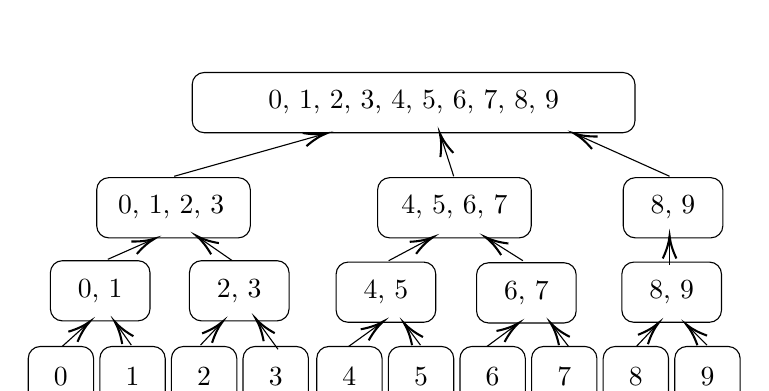
\begin{tikzpicture}[x=0.75pt,y=0.75pt,yscale=-1,xscale=1]
        %uncomment if require: \path (0,457); %set diagram left start at 0, and has height of 457

        %Rounded Rect [id:dp05055633926904224]
        \draw   (25,105.8) .. controls (25,102.6) and (27.6,100) .. (30.8,100) -- (67.2,100) .. controls (70.4,100) and (73,102.6) .. (73,105.8) -- (73,123.2) .. controls (73,126.4) and (70.4,129) .. (67.2,129) -- (30.8,129) .. controls (27.6,129) and (25,126.4) .. (25,123.2) -- cycle ;
        %Rounded Rect [id:dp14128108650523874]
        \draw   (14.33,147.13) .. controls (14.33,143.93) and (16.93,141.33) .. (20.13,141.33) -- (40.03,141.33) .. controls (43.24,141.33) and (45.83,143.93) .. (45.83,147.13) -- (45.83,164.53) .. controls (45.83,167.74) and (43.24,170.33) .. (40.03,170.33) -- (20.13,170.33) .. controls (16.93,170.33) and (14.33,167.74) .. (14.33,164.53) -- cycle ;
        %Rounded Rect [id:dp6850532710750563]
        \draw   (48.83,147.13) .. controls (48.83,143.93) and (51.43,141.33) .. (54.63,141.33) -- (74.53,141.33) .. controls (77.74,141.33) and (80.33,143.93) .. (80.33,147.13) -- (80.33,164.53) .. controls (80.33,167.74) and (77.74,170.33) .. (74.53,170.33) -- (54.63,170.33) .. controls (51.43,170.33) and (48.83,167.74) .. (48.83,164.53) -- cycle ;
        %Rounded Rect [id:dp49831794890726244]
        \draw   (83.33,147.13) .. controls (83.33,143.93) and (85.93,141.33) .. (89.13,141.33) -- (109.03,141.33) .. controls (112.24,141.33) and (114.83,143.93) .. (114.83,147.13) -- (114.83,164.53) .. controls (114.83,167.74) and (112.24,170.33) .. (109.03,170.33) -- (89.13,170.33) .. controls (85.93,170.33) and (83.33,167.74) .. (83.33,164.53) -- cycle ;
        %Rounded Rect [id:dp5704093284694525]
        \draw   (47.33,65.8) .. controls (47.33,62.6) and (49.93,60) .. (53.13,60) -- (115.53,60) .. controls (118.74,60) and (121.33,62.6) .. (121.33,65.8) -- (121.33,83.2) .. controls (121.33,86.4) and (118.74,89) .. (115.53,89) -- (53.13,89) .. controls (49.93,89) and (47.33,86.4) .. (47.33,83.2) -- cycle ;
        %Rounded Rect [id:dp06397000457352897]
        \draw   (117.83,147.13) .. controls (117.83,143.93) and (120.43,141.33) .. (123.63,141.33) -- (143.53,141.33) .. controls (146.74,141.33) and (149.33,143.93) .. (149.33,147.13) -- (149.33,164.53) .. controls (149.33,167.74) and (146.74,170.33) .. (143.53,170.33) -- (123.63,170.33) .. controls (120.43,170.33) and (117.83,167.74) .. (117.83,164.53) -- cycle ;
        %Rounded Rect [id:dp5625637649454729]
        \draw   (153.33,147.13) .. controls (153.33,143.93) and (155.93,141.33) .. (159.13,141.33) -- (179.03,141.33) .. controls (182.24,141.33) and (184.83,143.93) .. (184.83,147.13) -- (184.83,164.53) .. controls (184.83,167.74) and (182.24,170.33) .. (179.03,170.33) -- (159.13,170.33) .. controls (155.93,170.33) and (153.33,167.74) .. (153.33,164.53) -- cycle ;
        %Rounded Rect [id:dp10831678998895056]
        \draw   (187.83,147.13) .. controls (187.83,143.93) and (190.43,141.33) .. (193.63,141.33) -- (213.53,141.33) .. controls (216.74,141.33) and (219.33,143.93) .. (219.33,147.13) -- (219.33,164.53) .. controls (219.33,167.74) and (216.74,170.33) .. (213.53,170.33) -- (193.63,170.33) .. controls (190.43,170.33) and (187.83,167.74) .. (187.83,164.53) -- cycle ;
        %Rounded Rect [id:dp8486627726801472]
        \draw   (222.33,147.13) .. controls (222.33,143.93) and (224.93,141.33) .. (228.13,141.33) -- (248.03,141.33) .. controls (251.24,141.33) and (253.83,143.93) .. (253.83,147.13) -- (253.83,164.53) .. controls (253.83,167.74) and (251.24,170.33) .. (248.03,170.33) -- (228.13,170.33) .. controls (224.93,170.33) and (222.33,167.74) .. (222.33,164.53) -- cycle ;
        %Rounded Rect [id:dp16972516920971303]
        \draw   (256.83,147.13) .. controls (256.83,143.93) and (259.43,141.33) .. (262.63,141.33) -- (282.53,141.33) .. controls (285.74,141.33) and (288.33,143.93) .. (288.33,147.13) -- (288.33,164.53) .. controls (288.33,167.74) and (285.74,170.33) .. (282.53,170.33) -- (262.63,170.33) .. controls (259.43,170.33) and (256.83,167.74) .. (256.83,164.53) -- cycle ;
        %Rounded Rect [id:dp6840956909277642]
        \draw   (291.33,147.13) .. controls (291.33,143.93) and (293.93,141.33) .. (297.13,141.33) -- (317.03,141.33) .. controls (320.24,141.33) and (322.83,143.93) .. (322.83,147.13) -- (322.83,164.53) .. controls (322.83,167.74) and (320.24,170.33) .. (317.03,170.33) -- (297.13,170.33) .. controls (293.93,170.33) and (291.33,167.74) .. (291.33,164.53) -- cycle ;
        %Rounded Rect [id:dp1958758392948894]
        \draw   (325.83,147.13) .. controls (325.83,143.93) and (328.43,141.33) .. (331.63,141.33) -- (351.53,141.33) .. controls (354.74,141.33) and (357.33,143.93) .. (357.33,147.13) -- (357.33,164.53) .. controls (357.33,167.74) and (354.74,170.33) .. (351.53,170.33) -- (331.63,170.33) .. controls (328.43,170.33) and (325.83,167.74) .. (325.83,164.53) -- cycle ;
        %Rounded Rect [id:dp6436545397528568]
        \draw   (92,105.8) .. controls (92,102.6) and (94.6,100) .. (97.8,100) -- (134.2,100) .. controls (137.4,100) and (140,102.6) .. (140,105.8) -- (140,123.2) .. controls (140,126.4) and (137.4,129) .. (134.2,129) -- (97.8,129) .. controls (94.6,129) and (92,126.4) .. (92,123.2) -- cycle ;
        %Rounded Rect [id:dp3544971098617955]
        \draw   (162.67,106.47) .. controls (162.67,103.26) and (165.26,100.67) .. (168.47,100.67) -- (204.87,100.67) .. controls (208.07,100.67) and (210.67,103.26) .. (210.67,106.47) -- (210.67,123.87) .. controls (210.67,127.07) and (208.07,129.67) .. (204.87,129.67) -- (168.47,129.67) .. controls (165.26,129.67) and (162.67,127.07) .. (162.67,123.87) -- cycle ;
        %Rounded Rect [id:dp6212249066962128]
        \draw   (230.33,106.8) .. controls (230.33,103.6) and (232.93,101) .. (236.13,101) -- (272.53,101) .. controls (275.74,101) and (278.33,103.6) .. (278.33,106.8) -- (278.33,124.2) .. controls (278.33,127.4) and (275.74,130) .. (272.53,130) -- (236.13,130) .. controls (232.93,130) and (230.33,127.4) .. (230.33,124.2) -- cycle ;
        %Rounded Rect [id:dp24757598236323686]
        \draw   (300.33,106.47) .. controls (300.33,103.26) and (302.93,100.67) .. (306.13,100.67) -- (342.53,100.67) .. controls (345.74,100.67) and (348.33,103.26) .. (348.33,106.47) -- (348.33,123.87) .. controls (348.33,127.07) and (345.74,129.67) .. (342.53,129.67) -- (306.13,129.67) .. controls (302.93,129.67) and (300.33,127.07) .. (300.33,123.87) -- cycle ;
        %Rounded Rect [id:dp8713238483193051]
        \draw   (182.67,65.8) .. controls (182.67,62.6) and (185.26,60) .. (188.47,60) -- (250.87,60) .. controls (254.07,60) and (256.67,62.6) .. (256.67,65.8) -- (256.67,83.2) .. controls (256.67,86.4) and (254.07,89) .. (250.87,89) -- (188.47,89) .. controls (185.26,89) and (182.67,86.4) .. (182.67,83.2) -- cycle ;
        %Rounded Rect [id:dp8093819546801242]
        \draw   (93.33,15.13) .. controls (93.33,11.93) and (95.93,9.33) .. (99.13,9.33) -- (300.87,9.33) .. controls (304.07,9.33) and (306.67,11.93) .. (306.67,15.13) -- (306.67,32.53) .. controls (306.67,35.74) and (304.07,38.33) .. (300.87,38.33) -- (99.13,38.33) .. controls (95.93,38.33) and (93.33,35.74) .. (93.33,32.53) -- cycle ;
        %Rounded Rect [id:dp44931018514343335]
        \draw   (301,65.8) .. controls (301,62.6) and (303.6,60) .. (306.8,60) -- (343.2,60) .. controls (346.4,60) and (349,62.6) .. (349,65.8) -- (349,83.2) .. controls (349,86.4) and (346.4,89) .. (343.2,89) -- (306.8,89) .. controls (303.6,89) and (301,86.4) .. (301,83.2) -- cycle ;
        %Straight Lines [id:da27872296512255956]
        \draw    (30.67,141.33) -- (42.51,130.67) ;
        \draw [shift={(44,129.33)}, rotate = 498.01] [color={rgb, 255:red, 0; green, 0; blue, 0 }  ][line width=0.75]    (10.93,-3.29) .. controls (6.95,-1.4) and (3.31,-0.3) .. (0,0) .. controls (3.31,0.3) and (6.95,1.4) .. (10.93,3.29)   ;

        %Straight Lines [id:da597234089010694]
        \draw    (64,140.67) -- (57.15,130.97) ;
        \draw [shift={(56,129.33)}, rotate = 414.78] [color={rgb, 255:red, 0; green, 0; blue, 0 }  ][line width=0.75]    (10.93,-3.29) .. controls (6.95,-1.4) and (3.31,-0.3) .. (0,0) .. controls (3.31,0.3) and (6.95,1.4) .. (10.93,3.29)   ;

        %Straight Lines [id:da4850782748643834]
        \draw    (97.33,140.67) -- (106.63,130.79) ;
        \draw [shift={(108,129.33)}, rotate = 493.26] [color={rgb, 255:red, 0; green, 0; blue, 0 }  ][line width=0.75]    (10.93,-3.29) .. controls (6.95,-1.4) and (3.31,-0.3) .. (0,0) .. controls (3.31,0.3) and (6.95,1.4) .. (10.93,3.29)   ;

        %Straight Lines [id:da7930566056169013]
        \draw    (134.67,142.67) -- (125.18,129.62) ;
        \draw [shift={(124,128)}, rotate = 413.97] [color={rgb, 255:red, 0; green, 0; blue, 0 }  ][line width=0.75]    (10.93,-3.29) .. controls (6.95,-1.4) and (3.31,-0.3) .. (0,0) .. controls (3.31,0.3) and (6.95,1.4) .. (10.93,3.29)   ;

        %Straight Lines [id:da06697954280577867]
        \draw    (168.67,141.33) -- (183.71,130.5) ;
        \draw [shift={(185.33,129.33)}, rotate = 504.25] [color={rgb, 255:red, 0; green, 0; blue, 0 }  ][line width=0.75]    (10.93,-3.29) .. controls (6.95,-1.4) and (3.31,-0.3) .. (0,0) .. controls (3.31,0.3) and (6.95,1.4) .. (10.93,3.29)   ;

        %Straight Lines [id:da6534079236359922]
        \draw    (203.33,140.67) -- (196.53,131.6) ;
        \draw [shift={(195.33,130)}, rotate = 413.13] [color={rgb, 255:red, 0; green, 0; blue, 0 }  ][line width=0.75]    (10.93,-3.29) .. controls (6.95,-1.4) and (3.31,-0.3) .. (0,0) .. controls (3.31,0.3) and (6.95,1.4) .. (10.93,3.29)   ;

        %Straight Lines [id:da4482322713178277]
        \draw    (235.33,141.33) -- (249.06,131.19) ;
        \draw [shift={(250.67,130)}, rotate = 503.53] [color={rgb, 255:red, 0; green, 0; blue, 0 }  ][line width=0.75]    (10.93,-3.29) .. controls (6.95,-1.4) and (3.31,-0.3) .. (0,0) .. controls (3.31,0.3) and (6.95,1.4) .. (10.93,3.29)   ;

        %Straight Lines [id:da16086535271258762]
        \draw    (274.67,141.33) -- (267.21,131.59) ;
        \draw [shift={(266,130)}, rotate = 412.59000000000003] [color={rgb, 255:red, 0; green, 0; blue, 0 }  ][line width=0.75]    (10.93,-3.29) .. controls (6.95,-1.4) and (3.31,-0.3) .. (0,0) .. controls (3.31,0.3) and (6.95,1.4) .. (10.93,3.29)   ;

        %Straight Lines [id:da8935727309957442]
        \draw    (307.33,141.33) -- (316.63,131.46) ;
        \draw [shift={(318,130)}, rotate = 493.26] [color={rgb, 255:red, 0; green, 0; blue, 0 }  ][line width=0.75]    (10.93,-3.29) .. controls (6.95,-1.4) and (3.31,-0.3) .. (0,0) .. controls (3.31,0.3) and (6.95,1.4) .. (10.93,3.29)   ;

        %Straight Lines [id:da12427188024632208]
        \draw    (341.33,140.67) -- (332.75,132.08) ;
        \draw [shift={(331.33,130.67)}, rotate = 405] [color={rgb, 255:red, 0; green, 0; blue, 0 }  ][line width=0.75]    (10.93,-3.29) .. controls (6.95,-1.4) and (3.31,-0.3) .. (0,0) .. controls (3.31,0.3) and (6.95,1.4) .. (10.93,3.29)   ;

        %Straight Lines [id:da23222234042969503]
        \draw    (52.67,99.33) -- (73.5,90.14) ;
        \draw [shift={(75.33,89.33)}, rotate = 516.19] [color={rgb, 255:red, 0; green, 0; blue, 0 }  ][line width=0.75]    (10.93,-3.29) .. controls (6.95,-1.4) and (3.31,-0.3) .. (0,0) .. controls (3.31,0.3) and (6.95,1.4) .. (10.93,3.29)   ;

        %Straight Lines [id:da9082685186856525]
        \draw    (112.67,100) -- (96.98,89.14) ;
        \draw [shift={(95.33,88)}, rotate = 394.7] [color={rgb, 255:red, 0; green, 0; blue, 0 }  ][line width=0.75]    (10.93,-3.29) .. controls (6.95,-1.4) and (3.31,-0.3) .. (0,0) .. controls (3.31,0.3) and (6.95,1.4) .. (10.93,3.29)   ;

        %Straight Lines [id:da035871989319939956]
        \draw    (188,100) -- (207.57,89.6) ;
        \draw [shift={(209.33,88.67)}, rotate = 512.02] [color={rgb, 255:red, 0; green, 0; blue, 0 }  ][line width=0.75]    (10.93,-3.29) .. controls (6.95,-1.4) and (3.31,-0.3) .. (0,0) .. controls (3.31,0.3) and (6.95,1.4) .. (10.93,3.29)   ;

        %Straight Lines [id:da9798888674185477]
        \draw    (252.67,100) -- (236.36,89.73) ;
        \draw [shift={(234.67,88.67)}, rotate = 392.2] [color={rgb, 255:red, 0; green, 0; blue, 0 }  ][line width=0.75]    (10.93,-3.29) .. controls (6.95,-1.4) and (3.31,-0.3) .. (0,0) .. controls (3.31,0.3) and (6.95,1.4) .. (10.93,3.29)   ;

        %Straight Lines [id:da5655371856053]
        \draw    (323.33,102) -- (323.33,90) ;
        \draw [shift={(323.33,88)}, rotate = 450] [color={rgb, 255:red, 0; green, 0; blue, 0 }  ][line width=0.75]    (10.93,-3.29) .. controls (6.95,-1.4) and (3.31,-0.3) .. (0,0) .. controls (3.31,0.3) and (6.95,1.4) .. (10.93,3.29)   ;

        %Straight Lines [id:da5307091955398382]
        \draw    (84.67,59.33) -- (156.07,39.21) ;
        \draw [shift={(158,38.67)}, rotate = 524.26] [color={rgb, 255:red, 0; green, 0; blue, 0 }  ][line width=0.75]    (10.93,-3.29) .. controls (6.95,-1.4) and (3.31,-0.3) .. (0,0) .. controls (3.31,0.3) and (6.95,1.4) .. (10.93,3.29)   ;

        %Straight Lines [id:da23705174012369667]
        \draw    (219.33,59.33) -- (213.28,40.57) ;
        \draw [shift={(212.67,38.67)}, rotate = 432.12] [color={rgb, 255:red, 0; green, 0; blue, 0 }  ][line width=0.75]    (10.93,-3.29) .. controls (6.95,-1.4) and (3.31,-0.3) .. (0,0) .. controls (3.31,0.3) and (6.95,1.4) .. (10.93,3.29)   ;

        %Straight Lines [id:da10111862824392315]
        \draw    (323.33,59.33) -- (279.16,39.49) ;
        \draw [shift={(277.33,38.67)}, rotate = 384.19] [color={rgb, 255:red, 0; green, 0; blue, 0 }  ][line width=0.75]    (10.93,-3.29) .. controls (6.95,-1.4) and (3.31,-0.3) .. (0,0) .. controls (3.31,0.3) and (6.95,1.4) .. (10.93,3.29)   ;


        % Text Node
        \draw (30.08,155.83) node  [align=left] {0};
        % Text Node
        \draw (64.58,155.83) node  [align=left] {1};
        % Text Node
        \draw (99.08,155.83) node  [align=left] {2};
        % Text Node
        \draw (133.58,155.83) node  [align=left] {3};
        % Text Node
        \draw (169.08,155.83) node  [align=left] {4};
        % Text Node
        \draw (203.58,155.83) node  [align=left] {5};
        % Text Node
        \draw (238.08,155.83) node  [align=left] {6};
        % Text Node
        \draw (272.58,155.83) node  [align=left] {7};
        % Text Node
        \draw (307.08,155.83) node  [align=left] {8};
        % Text Node
        \draw (341.58,155.83) node  [align=left] {9};
        % Text Node
        \draw (49,114.5) node  [align=left] {0, 1};
        % Text Node
        \draw (116,114.5) node  [align=left] {2, 3};
        % Text Node
        \draw (186.67,115.17) node  [align=left] {4, 5};
        % Text Node
        \draw (254.33,115.5) node  [align=left] {6, 7};
        % Text Node
        \draw (324.33,115.17) node  [align=left] {8, 9};
        % Text Node
        \draw (83.17,74.5) node  [align=left] {0, 1, 2, 3};
        % Text Node
        \draw (219.67,74.5) node  [align=left] {4, 5, 6, 7};
        % Text Node
        \draw (200,23.83) node  [align=left] {0, 1, 2, 3, 4, 5, 6, 7, 8, 9};
        % Text Node
        \draw (325,74.5) node  [align=left] {8, 9};


    \end{tikzpicture}

    \caption{Hierarchy for the score attribute}\label{fig:score_hierarchy}
\end{figure}

This is a valid generalization hierarchy, because each partition at the leaf nodes contain only a single element, the top level contains a single set with all elements and finally the union of all sets on every level of the hierarchy is equal to the full domain of values.

Let's calculate the generalization cost for the first two rows.

In order to transform the values of the first attribute pair \((4, 7)\) into the same partition, they need to be generalized exactly two times until their values become [4, 5, 6, 7].
This means, that the unscaled generalization cost for the score attribute \(h_{a,b}(0)=2\).
The scaling factor corresponds to the highest level in the hierarchy: \(l_0=3\), so the scaled generalization cost will be \(h_{a,b}(0)/l_0=2/3\).

The edge cost between the nodes representing the first two rows will be the sum of the scaled generalization costs of \((4, 7)\), \((C-,B+)\) and \((male, male)\).
Using the grade hierarchy introduced in Chapter~\ref{subsec:data_model} in figure~\ref{fig:grades-hierarchy} and considering that the values of the gender attribute are already in the same partition, so their generalization cost will be 0:
\begin{center}
    \(w(e_{a,b})=2/3+1+0=5/3\).
\end{center}


If we repeat the above calculation for each row pair, we can determine the cost-graph for this table.
This process is left to the reader, but after finishing it the resulting graph should be isomorphic to the graph on figure~\ref{fig:cost_graph}.

\vspace{\baselineskip}
\begin{figure}[H]

    \centering
    \tikzset{every picture/.style={line width=0.75pt}} %set default line width to 0.75pt

    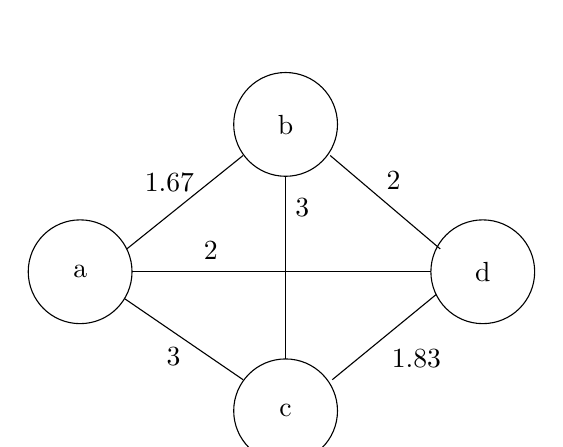
\begin{tikzpicture}[x=0.75pt,y=0.75pt,yscale=-1,xscale=1]
        %uncomment if require: \path (0,300); %set diagram left start at 0, and has height of 300

        %Shape: Circle [id:dp14719016101017623]
        \draw   (111,126) .. controls (111,112.19) and (122.19,101) .. (136,101) .. controls (149.81,101) and (161,112.19) .. (161,126) .. controls (161,139.81) and (149.81,151) .. (136,151) .. controls (122.19,151) and (111,139.81) .. (111,126) -- cycle ;
        %Shape: Circle [id:dp637969227645387]
        \draw   (210,55) .. controls (210,41.19) and (221.19,30) .. (235,30) .. controls (248.81,30) and (260,41.19) .. (260,55) .. controls (260,68.81) and (248.81,80) .. (235,80) .. controls (221.19,80) and (210,68.81) .. (210,55) -- cycle ;
        %Shape: Circle [id:dp16996306115691606]
        \draw   (210,193) .. controls (210,179.19) and (221.19,168) .. (235,168) .. controls (248.81,168) and (260,179.19) .. (260,193) .. controls (260,206.81) and (248.81,218) .. (235,218) .. controls (221.19,218) and (210,206.81) .. (210,193) -- cycle ;
        %Shape: Circle [id:dp4723269788902422]
        \draw   (305,126) .. controls (305,112.19) and (316.19,101) .. (330,101) .. controls (343.81,101) and (355,112.19) .. (355,126) .. controls (355,139.81) and (343.81,151) .. (330,151) .. controls (316.19,151) and (305,139.81) .. (305,126) -- cycle ;
        %Straight Lines [id:da43115389914855107]
        \draw    (158.5,115) -- (214.5,70) ;


        %Straight Lines [id:da3262134359528708]
        \draw    (257.5,178) -- (307.5,137) ;


        %Straight Lines [id:da6644861489456326]
        \draw    (235,168) -- (235,80) ;


        %Straight Lines [id:da44726258546505226]
        \draw    (157.5,139) -- (214.5,178) ;


        %Straight Lines [id:da17516578825824003]
        \draw    (309.5,115) -- (256.5,70) ;


        %Straight Lines [id:da25861424028019475]
        \draw    (161,126) -- (305,126) ;



        % Text Node
        \draw (136,126) node  [align=left] {a};
        % Text Node
        \draw (235,55) node  [align=left] {b};
        % Text Node
        \draw (235,193) node  [align=left] {c};
        % Text Node
        \draw (330,126) node  [align=left] {d};
        % Text Node
        \draw (179,83) node  [align=left] {1.67};
        % Text Node
        \draw (181,167) node  [align=left] {3};
        % Text Node
        \draw (199,116) node  [align=left] {2};
        % Text Node
        \draw (243,95) node  [align=left] {3};
        % Text Node
        \draw (287,82) node  [align=left] {2};
        % Text Node
        \draw (298,168) node  [align=left] {1.83};


    \end{tikzpicture}

    \caption{Example cost-graph}\label{fig:cost_graph}
\end{figure}

\subsection{A note on the limitations of the graph representation}\label{subsec:a-note-on-the-limitations-of-the-graph-representation}

Unfortunately the graph representation has some limitations, as the original authors also note in their article~\cite{aggarwal}.
When the input data table is transformed into its graph equivalent, some information is lost which results in the algorithm only being able to achieve the \(\mathcal{O}(k)\) approximation factor.

This can be demonstrated by constructing two input tables on a binary alphabet (\(\Sigma={0,1}\)) for a given \textit{k} value in a way, that the optimal anonymization cost and the total cost incurred by the graph representation differs by a factor of \(\mathcal{O}(k)\):

Let \(l=2^{k-2}\).

\paragraph{Table A} should be \(k \times kl\), and for each row \textit{i} contains the value \textbf{1} in positions \([(i-1)l+1 \dots il]\) and \textbf{0} otherwise.
The anonymization cost for this table is \(k^2 l\).

\vspace{\baselineskip}
\begin{figure}[H]
    \centering
    \(
    \begin{pmatrix}
        1 & 1 & 0 & 0 & 0 & 0 \\
        0 & 0 & 1 & 1 & 0 & 0 \\
        0 & 0 & 0 & 0 & 1 & 1
    \end{pmatrix}
    \)
    \caption{Example for type A table and k=3, l=2}\label{fig:graph_limit_A}
\end{figure}

\paragraph{Table B} should be \(k \times 4l\).
Its \(i^{th}\) row is broken down into \(2^i\) equal-sized blocks.
Every value in odd blocks is \textbf{0}, and every value in even blocks is \textbf{1}.
The anonymization cost for this table is \(4kl\).

\vspace{\baselineskip}
\begin{figure}[H]
    \centering
    \(
    \begin{pmatrix}
        0 & 0 & 0 & 0 & 1 & 1 & 1 & 1 \\
        0 & 0 & 1 & 1 & 0 & 0 & 1 & 1 \\
        0 & 1 & 0 & 1 & 0 & 1 & 0 & 1
    \end{pmatrix}
    \)
    \caption{Example for type B table and k=3, l=2}\label{fig:graph_limit_B}
\end{figure}

Note, that both tables are represented by a k-clique with all edge costs being \(2l=2^{k-1}\), while their respective anonymization cost differs by exactly \(\mathcal{O}(k)\).

\vspace{\baselineskip}
\begin{figure}[H]
    \centering


    \tikzset{every picture/.style={line width=0.75pt}} %set default line width to 0.75pt

    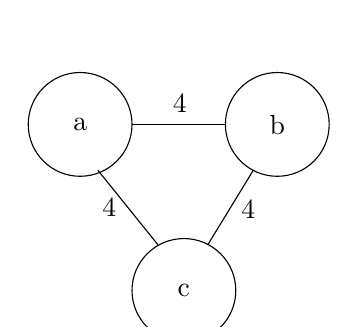
\begin{tikzpicture}[x=0.75pt,y=0.75pt,yscale=-1,xscale=1]
        %uncomment if require: \path (0,300); %set diagram left start at 0, and has height of 300

        %Shape: Circle [id:dp058849468526875004]
        \draw   (59,60) .. controls (59,46.19) and (70.19,35) .. (84,35) .. controls (97.81,35) and (109,46.19) .. (109,60) .. controls (109,73.81) and (97.81,85) .. (84,85) .. controls (70.19,85) and (59,73.81) .. (59,60) -- cycle ;
        %Shape: Circle [id:dp11003911798399524]
        \draw   (154,60) .. controls (154,46.19) and (165.19,35) .. (179,35) .. controls (192.81,35) and (204,46.19) .. (204,60) .. controls (204,73.81) and (192.81,85) .. (179,85) .. controls (165.19,85) and (154,73.81) .. (154,60) -- cycle ;
        %Shape: Circle [id:dp7927588085940704]
        \draw   (109,140) .. controls (109,126.19) and (120.19,115) .. (134,115) .. controls (147.81,115) and (159,126.19) .. (159,140) .. controls (159,153.81) and (147.81,165) .. (134,165) .. controls (120.19,165) and (109,153.81) .. (109,140) -- cycle ;
        %Straight Lines [id:da30216407066666995]
        \draw    (109,60) -- (154,60) ;


        %Straight Lines [id:da024128079077286868]
        \draw    (92.5,82) -- (121.5,118) ;


        %Straight Lines [id:da48310889364666654]
        \draw    (167.5,82) -- (145.5,118) ;



        % Text Node
        \draw (84,60) node  [align=left] {a};
        % Text Node
        \draw (179,60) node  [align=left] {b};
        % Text Node
        \draw (134,140) node  [align=left] {c};
        % Text Node
        \draw (132,50) node  [align=left] {4};
        % Text Node
        \draw (98,100) node  [align=left] {4};
        % Text Node
        \draw (165,101) node  [align=left] {4};


    \end{tikzpicture}

    \caption{Graph representation of both Table A and Table B}\label{fig:graph_limit_graph}

\end{figure}

\subsection{Forest building algorithm}\label{subsec:forest-building-algorithm}

The next step in the overall k-anonymity algorithm is to produce a forest. (Section~\ref{sec:algorithm_outline}) We will now use the nodes and calculated weights from the cost-graph, but in this step we will be constructing a directed graph which will ultimately be used to represent a partitioning of the original row vectors.

\paragraph{Algorithm} \textsc{Forest building}~\cite{aggarwal}

Invariant:
\begin{itemize}
    \item The chosen edges do not create any cycle.
    \item The out-degree of each vertex is at most one.
\end{itemize}

Steps:
\begin{enumerate}
    \item Start with an empty edge set so that each vertex is in its own connected component.
    \item Repeat until all components are of size at least \textit{k}: \par
    Pick any component \textit{T} having size smaller than \textit{k}.
    Let \textit{u} be a vertex in \textit{T} without any outgoing edges.
    Since there are at most \(k-2\) other vertices in \textit{T}, one of the \(k-1\) \emph{nearest neighbors} of \textit{u}, say \textit{v}, must lie outside \textit{T}.
    We add the edge \(\vec{uv}\) to the forest. \textit{(Observe that this step does not violate any of the invariants.)}
\end{enumerate}

\vspace{\baselineskip}

In simple terms we start from the original graph without any edges.
In every step we extend a selected tree (\(size < k\)) in the forest.
We add a new vertex to the tree by selecting an \textit{u} ``leaf'' (without any outgoing edges) in the current tree, and connecting it with its lowest cost neighbor \textit{v}.

\paragraph{Lemma} The forest produced by the Forest building algorithm has a minimum tree size at least \textit{k} and has cost at most \textit{OPT}, where \textit{OPT} denotes the cost of an optimal k-anonymity solution~\cite{aggarwal}.

\paragraph{Example} Forest building (\(k=3\))\label{sec:forest_building_example}

For this example let's assume that the cost-graph has already been computed from the input table, and is isomorph to the graph shown on figure~\ref{fig:forest_cost_graph}.

\vspace{\baselineskip}
\begin{figure}[H]
    \centering
    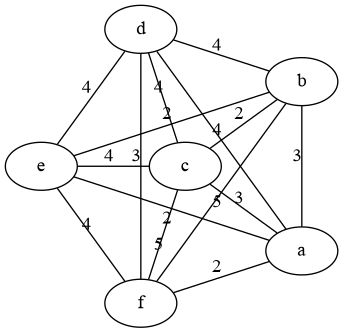
\includegraphics[width=200pt]{forest-example-cost.png}
    \caption{Example cost graph}\label{fig:forest_cost_graph}
\end{figure}

The starting position has all nodes in their separate component.
From there, the steps of the algorithm can be traced on figure~\ref{fig:forest_partitioning}.

\begin{figure}
    \centering
    \subfloat[Step 1]{{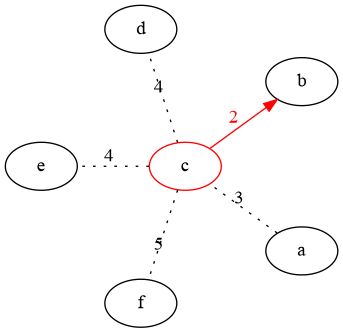
\includegraphics[width=6cm]{images/forest-example-1.png} }}
    \vspace{0.6cm}
    \subfloat[Step 2]{{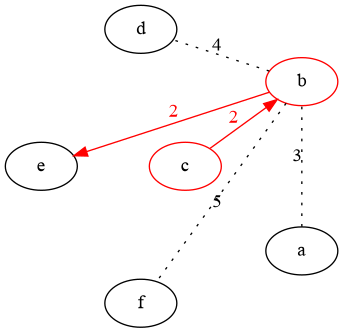
\includegraphics[width=6cm]{images/forest-example-2.png} }}
    \vspace{0.6cm}
    \subfloat[Step 3]{{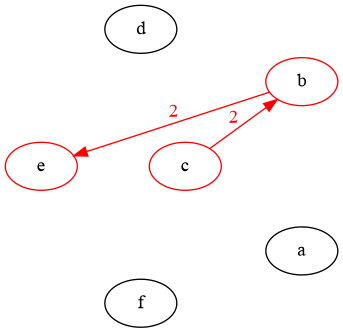
\includegraphics[width=6cm]{images/forest-example-3.png} }}
    \vspace{0.6cm}
    \subfloat[Step 4]{{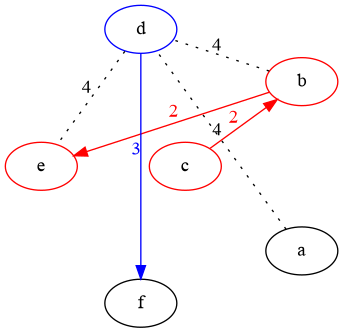
\includegraphics[width=6cm]{images/forest-example-4.png} }}
    \vspace{0.6cm}
    \subfloat[Step 5]{{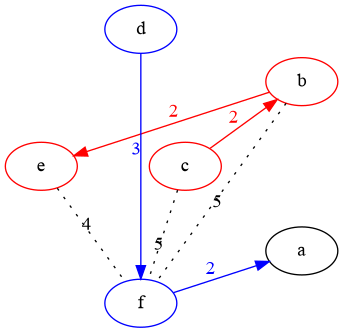
\includegraphics[width=6cm]{images/forest-example-5.png} }}
    \vspace{0.6cm}
    \subfloat[Step 6]{{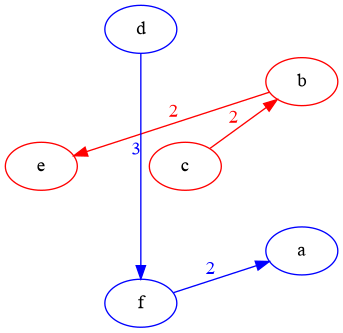
\includegraphics[width=6cm]{images/forest-example-6.png} }}
    \caption{Forest Building Algorithm}\label{fig:forest_partitioning}
\end{figure}

The forest building algorithm starts from an empty edge set.
Each node is in a separate component.
Since at this point the size of each component is smaller than \textit{k}, we pick a component to extend at random.

In Step 1 of the example we picked the component which contains the \textit{c} node.
Inspecting the outgoing edges we find that the closest one is the edge going to \textit{b}.
In Step 2 we continue extending the same component, since its size is still under the threshold.
Node \textit{b} is now part of the component, and has no outgoing edges, so we try to find an outgoing edge from that.
Closest is the component containing \textit{e}, so we add it.

At this point, the component's size has reached \(k=3\), so we move on to another component to extend.
In Step 4 we have picked \textit{d}.
Note, at this point when considering the possible edges we also considered edges between \textit{d} and nodes in the previously created component (\textit{b} and \textit{e}).
This is an example of how this part of the algorithm could end up with component sizes greater than \textit{k}.
In this example however, the closest neighbor is \textit{f}, and by Step 6 we can cleanly finish the partitioning with two 3-node partitions.

\subsection{Algorithm to decompose oversized components}\label{subsec:algorithm-to-decompose-oversized-components}

In the example in Section~\ref{sec:forest_building_example} we fortunately ended up with two perfectly sized components, which defined a good partitioning for anonymization.
This will not always be the case however, and there may be oversized components in the forest.

In this section we show an algorithm to break any component with size \(s \ge \max \{ 2k-1, 3k-5 \} \) into two components each of size at least \textit{k}. (The following algorithm treats the component as an \emph{undirected} graph.)

\paragraph{Algorithm} \textsc{Decompose component}~\cite{aggarwal}

\begin{enumerate}
    \item Pick any vertex \textit{u} as the candidate vertex.
    \item Root the tree at the candidate vertex \textit{u}.
    Let U be the set of sub-trees rooted at the children of \textit{u}.
    Let the size of the largest subtree of \textit{u} be \( \phi \), rooted at vertex \textit{v}. (See figure~\ref{fig:decompose}) If \(s-\phi \ge k-1\), then we do one of the following partition and terminate:
    \begin{enumerate}
        \item[A.] If \(\phi \ge k\) and \(s-\phi \ge k\), then partition the tree into the largest subtree and the rest.
        \item[B.] If \(s-\phi = k-1\), partition the tree into a component containing the subtrees rooted at the children of \textit{v} and the rest.
        To connect the children of \textit{v} create a \emph{Steiner's Vertex} (see below).
        \item[C.] If \(\phi = k-1\), then partition into a component containing the subtree rooted at \textit{v} along with the vertex \textit{u} and the rest.
        In order to connect the children of \textit{u} create a \emph{Steiner's Vertex}.
        \item[D.] Otherwise, all subtrees have size at most \(k-2\).
        In this case, we create an empty partition and keep adding subtrees of \textit{u} to it until the first time its size becomes at least \(k-1\).
        Put the remaining subtrees into the other partition.
        If one of the partitions has size equal to \(k-1\), add \textit{u} to that partition.
        Otherwise add \textit{u} to the first partition.
        In the partition not containing \textit{u} add a \emph{Steiner's Vertex} to keep it connected.
    \end{enumerate}
    \item Otherwise, pick \textit{v} as the new candidate vertex and go to Step 2.
\end{enumerate}

\vspace{\baselineskip}
\begin{figure}[H]
    \centering


    \tikzset{every picture/.style={line width=0.75pt}} %set default line width to 0.75pt

    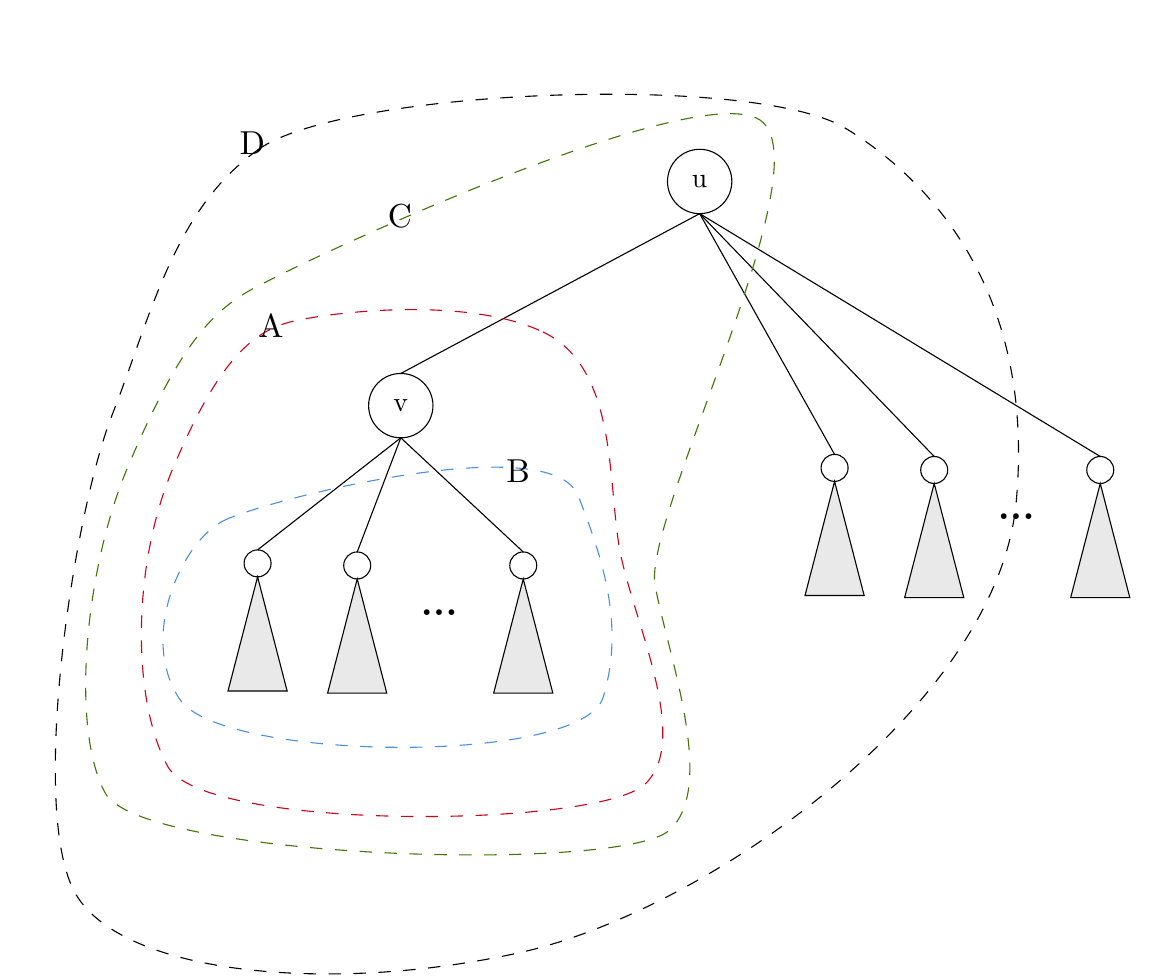
\begin{tikzpicture}[x=0.75pt,y=0.75pt,yscale=-1,xscale=1]
        %uncomment if require: \path (0,459); %set diagram left start at 0, and has height of 459

        %Shape: Circle [id:dp7711684678996311]
        \draw  [fill={rgb, 255:red, 255; green, 255; blue, 255 }  ,fill opacity=1 ] (302,48.5) .. controls (302,39.94) and (308.94,33) .. (317.5,33) .. controls (326.06,33) and (333,39.94) .. (333,48.5) .. controls (333,57.06) and (326.06,64) .. (317.5,64) .. controls (308.94,64) and (302,57.06) .. (302,48.5) -- cycle ;
        %Shape: Circle [id:dp8540052293183187]
        \draw  [fill={rgb, 255:red, 255; green, 255; blue, 255 }  ,fill opacity=1 ] (158,156.5) .. controls (158,147.94) and (164.94,141) .. (173.5,141) .. controls (182.06,141) and (189,147.94) .. (189,156.5) .. controls (189,165.06) and (182.06,172) .. (173.5,172) .. controls (164.94,172) and (158,165.06) .. (158,156.5) -- cycle ;
        %Shape: Circle [id:dp6767312206403671]
        \draw   (98,232.5) .. controls (98,228.91) and (100.91,226) .. (104.5,226) .. controls (108.09,226) and (111,228.91) .. (111,232.5) .. controls (111,236.09) and (108.09,239) .. (104.5,239) .. controls (100.91,239) and (98,236.09) .. (98,232.5) -- cycle ;
        %Shape: Triangle [id:dp6284155562718452]
        \draw  [fill={rgb, 255:red, 233; green, 233; blue, 233 }  ,fill opacity=1 ] (104.5,239) -- (118.75,294) -- (90.25,294) -- cycle ;
        %Shape: Circle [id:dp024913106678187136]
        \draw   (146,233.5) .. controls (146,229.91) and (148.91,227) .. (152.5,227) .. controls (156.09,227) and (159,229.91) .. (159,233.5) .. controls (159,237.09) and (156.09,240) .. (152.5,240) .. controls (148.91,240) and (146,237.09) .. (146,233.5) -- cycle ;
        %Shape: Triangle [id:dp11973699329342047]
        \draw  [fill={rgb, 255:red, 233; green, 233; blue, 233 }  ,fill opacity=1 ] (152.5,240) -- (166.75,295) -- (138.25,295) -- cycle ;
        %Shape: Circle [id:dp5828391286835717]
        \draw   (226,233.5) .. controls (226,229.91) and (228.91,227) .. (232.5,227) .. controls (236.09,227) and (239,229.91) .. (239,233.5) .. controls (239,237.09) and (236.09,240) .. (232.5,240) .. controls (228.91,240) and (226,237.09) .. (226,233.5) -- cycle ;
        %Shape: Triangle [id:dp2511681856589991]
        \draw  [fill={rgb, 255:red, 233; green, 233; blue, 233 }  ,fill opacity=1 ] (232.5,240) -- (246.75,295) -- (218.25,295) -- cycle ;
        %Shape: Circle [id:dp5623627355443772]
        \draw   (376,186.5) .. controls (376,182.91) and (378.91,180) .. (382.5,180) .. controls (386.09,180) and (389,182.91) .. (389,186.5) .. controls (389,190.09) and (386.09,193) .. (382.5,193) .. controls (378.91,193) and (376,190.09) .. (376,186.5) -- cycle ;
        %Shape: Triangle [id:dp39244508786141674]
        \draw  [fill={rgb, 255:red, 233; green, 233; blue, 233 }  ,fill opacity=1 ] (382.5,193) -- (396.75,248) -- (368.25,248) -- cycle ;
        %Shape: Circle [id:dp8178713595847904]
        \draw   (424,187.5) .. controls (424,183.91) and (426.91,181) .. (430.5,181) .. controls (434.09,181) and (437,183.91) .. (437,187.5) .. controls (437,191.09) and (434.09,194) .. (430.5,194) .. controls (426.91,194) and (424,191.09) .. (424,187.5) -- cycle ;
        %Shape: Triangle [id:dp3542102499533475]
        \draw  [fill={rgb, 255:red, 233; green, 233; blue, 233 }  ,fill opacity=1 ] (430.5,194) -- (444.75,249) -- (416.25,249) -- cycle ;
        %Shape: Circle [id:dp4483381477394748]
        \draw   (504,187.5) .. controls (504,183.91) and (506.91,181) .. (510.5,181) .. controls (514.09,181) and (517,183.91) .. (517,187.5) .. controls (517,191.09) and (514.09,194) .. (510.5,194) .. controls (506.91,194) and (504,191.09) .. (504,187.5) -- cycle ;
        %Shape: Triangle [id:dp4240387998981314]
        \draw  [fill={rgb, 255:red, 233; green, 233; blue, 233 }  ,fill opacity=1 ] (510.5,194) -- (524.75,249) -- (496.25,249) -- cycle ;
        %Straight Lines [id:da29060880873239037]
        \draw    (317.5,64) -- (173.5,141) ;


        %Straight Lines [id:da681996043601955]
        \draw    (317.5,64) -- (382.5,180) ;


        %Straight Lines [id:da7335165640252448]
        \draw    (317.5,64) -- (430.5,181) ;


        %Straight Lines [id:da39989551498039266]
        \draw    (317.5,64) -- (510.5,181) ;


        %Straight Lines [id:da27519719998677683]
        \draw    (104.5,226) -- (173.5,172) ;


        %Straight Lines [id:da1425001048459873]
        \draw    (152.5,227) -- (173.5,172) ;


        %Straight Lines [id:da8004516890426716]
        \draw    (232.5,227) -- (173.5,172) ;


        %Shape: Polygon Curved [id:ds10919181429761804]
        \draw  [color={rgb, 255:red, 208; green, 2; blue, 27 }  ,draw opacity=1 ][dash pattern={on 4.5pt off 4.5pt}] (242,121) .. controls (278,138) and (273,193) .. (279,226) .. controls (285,259) and (314,318) .. (291,339) .. controls (268,360) and (78,362) .. (61,330) .. controls (44,298) and (43.75,233.63) .. (64,186) .. controls (84.25,138.38) and (100,121) .. (121,116) .. controls (142,111) and (206,104) .. (242,121) -- cycle ;
        %Shape: Polygon Curved [id:ds3630985664957256]
        \draw  [color={rgb, 255:red, 74; green, 144; blue, 226 }  ,draw opacity=1 ][dash pattern={on 4.5pt off 4.5pt}] (88,212) .. controls (108,202) and (246,167) .. (259,200) .. controls (272,233) and (281,264) .. (271,297) .. controls (261,330) and (87,328) .. (67,298) .. controls (47,268) and (68,222) .. (88,212) -- cycle ;
        %Shape: Polygon Curved [id:ds6625985709394309]
        \draw  [color={rgb, 255:red, 65; green, 117; blue, 5 }  ,draw opacity=1 ][dash pattern={on 4.5pt off 4.5pt}] (345,18) .. controls (381,35) and (290,210) .. (296,243) .. controls (302,276) and (326,340) .. (303,361) .. controls (280,382) and (48,375) .. (31,343) .. controls (14,311) and (21.75,233.63) .. (42,186) .. controls (62.25,138.38) and (77,115) .. (99,102) .. controls (121,89) and (309,1) .. (345,18) -- cycle ;
        %Shape: Polygon Curved [id:ds5228551783856155]
        \draw  [color={rgb, 255:red, 0; green, 0; blue, 0 }  ,draw opacity=1 ][dash pattern={on 4.5pt off 4.5pt}] (105,33) .. controls (146,4) and (344,-4) .. (388,23) .. controls (432,50) and (479,105) .. (470,203) .. controls (461,301) and (321,400) .. (231,420) .. controls (141,440) and (40,431) .. (17,392) .. controls (-6,353) and (15.5,209) .. (34.5,160.75) .. controls (53.5,112.5) and (64,62) .. (105,33) -- cycle ;

        % Text Node
        \draw (317.5,48.5) node  [align=left] {u};
        % Text Node
        \draw (173.5,156.5) node  [align=left] {v};
        % Text Node
        \draw (192,256) node  [align=left] {\textbf{{\Large ...}}};
        % Text Node
        \draw (470,210) node  [align=left] {\textbf{{\Large ...}}};
        % Text Node
        \draw (111,118) node [scale=1.2] [align=left] {A};
        % Text Node
        \draw (230,188) node [scale=1.2] [align=left] {B};
        % Text Node
        \draw (173,65) node [scale=1.2] [align=left] {C};
        % Text Node
        \draw (102,30) node [scale=1.2] [align=left] {D};


    \end{tikzpicture}

    \caption{Different cut types for the decompose algorithm}\label{fig:decompose}
\end{figure}

\paragraph{The Steiner's Vertex} is a dummy vertex inserted to structurally hold the component together, but does not contribute to the size of the component during the algorithm.

\vspace{\baselineskip}
\begin{figure}[H]
    \centering




    \tikzset{every picture/.style={line width=0.75pt}} %set default line width to 0.75pt

    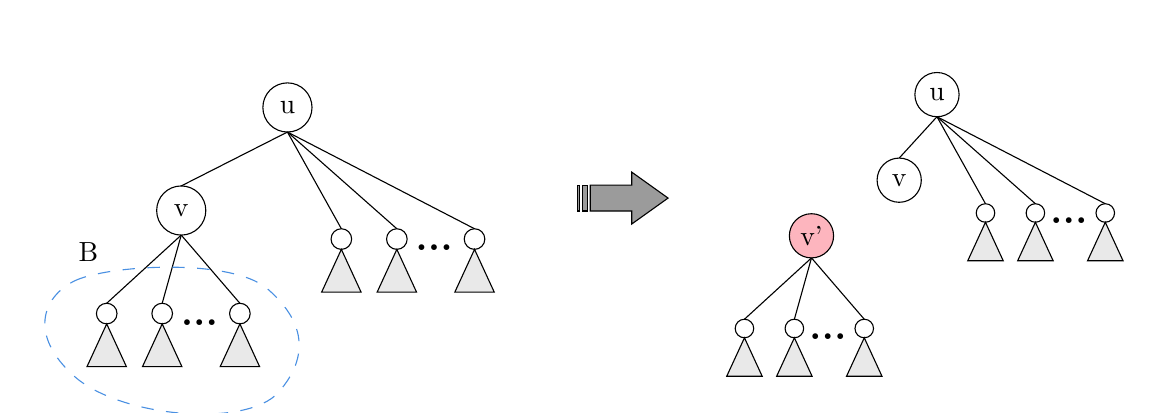
\begin{tikzpicture}[x=0.75pt,y=0.75pt,yscale=-1,xscale=1]
        %uncomment if require: \path (0,476); %set diagram left start at 0, and has height of 476

        %Shape: Ellipse [id:dp7890393065744103]
        \draw  [fill={rgb, 255:red, 255; green, 255; blue, 255 }  ,fill opacity=1 ] (124.52,36.84) .. controls (124.52,30.3) and (129.83,25) .. (136.36,25) .. controls (142.9,25) and (148.2,30.3) .. (148.2,36.84) .. controls (148.2,43.38) and (142.9,48.68) .. (136.36,48.68) .. controls (129.83,48.68) and (124.52,43.38) .. (124.52,36.84) -- cycle ;
        %Shape: Ellipse [id:dp618735643725828]
        \draw  [fill={rgb, 255:red, 255; green, 255; blue, 255 }  ,fill opacity=1 ] (73.35,86.49) .. controls (73.35,79.95) and (78.65,74.65) .. (85.19,74.65) .. controls (91.72,74.65) and (97.03,79.95) .. (97.03,86.49) .. controls (97.03,93.03) and (91.72,98.33) .. (85.19,98.33) .. controls (78.65,98.33) and (73.35,93.03) .. (73.35,86.49) -- cycle ;
        %Shape: Ellipse [id:dp4771904397826303]
        \draw   (44.32,136.14) .. controls (44.32,133.4) and (46.54,131.18) .. (49.28,131.18) .. controls (52.03,131.18) and (54.25,133.4) .. (54.25,136.14) .. controls (54.25,138.88) and (52.03,141.11) .. (49.28,141.11) .. controls (46.54,141.11) and (44.32,138.88) .. (44.32,136.14) -- cycle ;
        %Shape: Triangle [id:dp553752456661303]
        \draw  [fill={rgb, 255:red, 233; green, 233; blue, 233 }  ,fill opacity=1 ] (49.28,141.11) -- (58.78,161.73) -- (39.78,161.73) -- cycle ;

        %Shape: Ellipse [id:dp4582325504788667]
        \draw   (71.05,136.14) .. controls (71.05,133.4) and (73.28,131.18) .. (76.02,131.18) .. controls (78.76,131.18) and (80.98,133.4) .. (80.98,136.14) .. controls (80.98,138.88) and (78.76,141.11) .. (76.02,141.11) .. controls (73.28,141.11) and (71.05,138.88) .. (71.05,136.14) -- cycle ;
        %Shape: Triangle [id:dp5979831512805434]
        \draw  [fill={rgb, 255:red, 233; green, 233; blue, 233 }  ,fill opacity=1 ] (76.02,141.11) -- (85.52,161.73) -- (66.52,161.73) -- cycle ;

        %Shape: Ellipse [id:dp2963506198722945]
        \draw   (108.48,136.14) .. controls (108.48,133.4) and (110.71,131.18) .. (113.45,131.18) .. controls (116.19,131.18) and (118.41,133.4) .. (118.41,136.14) .. controls (118.41,138.88) and (116.19,141.11) .. (113.45,141.11) .. controls (110.71,141.11) and (108.48,138.88) .. (108.48,136.14) -- cycle ;
        %Shape: Triangle [id:dp6725407515322526]
        \draw  [fill={rgb, 255:red, 233; green, 233; blue, 233 }  ,fill opacity=1 ] (113.45,141.11) -- (122.95,161.73) -- (103.95,161.73) -- cycle ;

        %Shape: Circle [id:dp18476563967542958]
        \draw   (157.37,100.24) .. controls (157.37,97.5) and (159.59,95.28) .. (162.34,95.28) .. controls (165.08,95.28) and (167.3,97.5) .. (167.3,100.24) .. controls (167.3,102.98) and (165.08,105.21) .. (162.34,105.21) .. controls (159.59,105.21) and (157.37,102.98) .. (157.37,100.24) -- cycle ;
        %Shape: Triangle [id:dp466803100468395]
        \draw  [fill={rgb, 255:red, 233; green, 233; blue, 233 }  ,fill opacity=1 ] (162.34,105.21) -- (171.84,125.83) -- (152.83,125.83) -- cycle ;

        %Shape: Circle [id:dp5261729680381961]
        \draw   (184.11,100.24) .. controls (184.11,97.5) and (186.33,95.28) .. (189.07,95.28) .. controls (191.81,95.28) and (194.04,97.5) .. (194.04,100.24) .. controls (194.04,102.98) and (191.81,105.21) .. (189.07,105.21) .. controls (186.33,105.21) and (184.11,102.98) .. (184.11,100.24) -- cycle ;
        %Shape: Triangle [id:dp20443302728402402]
        \draw  [fill={rgb, 255:red, 233; green, 233; blue, 233 }  ,fill opacity=1 ] (189.07,105.21) -- (198.57,125.83) -- (179.57,125.83) -- cycle ;

        %Shape: Circle [id:dp720535105016272]
        \draw   (221.53,100.24) .. controls (221.53,97.5) and (223.76,95.28) .. (226.5,95.28) .. controls (229.24,95.28) and (231.46,97.5) .. (231.46,100.24) .. controls (231.46,102.98) and (229.24,105.21) .. (226.5,105.21) .. controls (223.76,105.21) and (221.53,102.98) .. (221.53,100.24) -- cycle ;
        %Shape: Triangle [id:dp7645667177753481]
        \draw  [fill={rgb, 255:red, 233; green, 233; blue, 233 }  ,fill opacity=1 ] (226.5,105.21) -- (236,125.83) -- (217,125.83) -- cycle ;

        %Straight Lines [id:da07079731319780569]
        \draw    (85.19,98.33) -- (49.28,131.18) ;


        %Straight Lines [id:da17784879908658002]
        \draw    (85.19,98.33) -- (76.02,131.18) ;


        %Straight Lines [id:da15620515081223996]
        \draw    (85.19,98.33) -- (113.45,131.18) ;


        %Straight Lines [id:da8013781550577805]
        \draw    (136.36,48.68) -- (85.19,74.65) ;


        %Straight Lines [id:da945479179142265]
        \draw    (136.36,48.68) -- (162.34,95.28) ;


        %Straight Lines [id:da1078430250095277]
        \draw    (136.36,48.68) -- (189.07,95.28) ;


        %Straight Lines [id:da2224960955888713]
        \draw    (136.36,48.68) -- (226.5,95.28) ;


        %Shape: Polygon Curved [id:ds3544729654410035]
        \draw  [color={rgb, 255:red, 74; green, 144; blue, 226 }  ,draw opacity=1 ][dash pattern={on 4.5pt off 4.5pt}] (33.62,120.48) .. controls (48.9,112.84) and (109.25,109.02) .. (126.82,124.3) .. controls (144.38,139.58) and (147.44,156.38) .. (132.16,173.95) .. controls (116.89,191.52) and (55.78,186.17) .. (33.62,166.31) .. controls (11.47,146.45) and (18.35,128.12) .. (33.62,120.48) -- cycle ;
        %Shape: Ellipse [id:dp6954675899235474]
        \draw  [fill={rgb, 255:red, 255; green, 255; blue, 255 }  ,fill opacity=1 ] (438.66,30.65) .. controls (438.66,24.77) and (443.43,20) .. (449.31,20) .. controls (455.19,20) and (459.96,24.77) .. (459.96,30.65) .. controls (459.96,36.53) and (455.19,41.3) .. (449.31,41.3) .. controls (443.43,41.3) and (438.66,36.53) .. (438.66,30.65) -- cycle ;
        %Shape: Ellipse [id:dp2597907901086436]
        \draw  [fill={rgb, 255:red, 253; green, 181; blue, 190 }  ,fill opacity=1 ] (378.19,98.68) .. controls (378.19,92.79) and (382.96,88.03) .. (388.84,88.03) .. controls (394.72,88.03) and (399.49,92.79) .. (399.49,98.68) .. controls (399.49,104.56) and (394.72,109.33) .. (388.84,109.33) .. controls (382.96,109.33) and (378.19,104.56) .. (378.19,98.68) -- cycle ;
        %Shape: Ellipse [id:dp5664348554601168]
        \draw   (352.08,143.34) .. controls (352.08,140.87) and (354.08,138.87) .. (356.55,138.87) .. controls (359.01,138.87) and (361.01,140.87) .. (361.01,143.34) .. controls (361.01,145.81) and (359.01,147.81) .. (356.55,147.81) .. controls (354.08,147.81) and (352.08,145.81) .. (352.08,143.34) -- cycle ;
        %Shape: Triangle [id:dp7826763983443301]
        \draw  [fill={rgb, 255:red, 233; green, 233; blue, 233 }  ,fill opacity=1 ] (356.55,147.81) -- (365.09,166.36) -- (348,166.36) -- cycle ;

        %Shape: Ellipse [id:dp19804184401026292]
        \draw   (376.13,143.34) .. controls (376.13,140.87) and (378.13,138.87) .. (380.6,138.87) .. controls (383.06,138.87) and (385.06,140.87) .. (385.06,143.34) .. controls (385.06,145.81) and (383.06,147.81) .. (380.6,147.81) .. controls (378.13,147.81) and (376.13,145.81) .. (376.13,143.34) -- cycle ;
        %Shape: Triangle [id:dp1257939998917028]
        \draw  [fill={rgb, 255:red, 233; green, 233; blue, 233 }  ,fill opacity=1 ] (380.6,147.81) -- (389.14,166.36) -- (372.05,166.36) -- cycle ;

        %Shape: Ellipse [id:dp6791067615266415]
        \draw   (409.8,143.34) .. controls (409.8,140.87) and (411.8,138.87) .. (414.27,138.87) .. controls (416.73,138.87) and (418.73,140.87) .. (418.73,143.34) .. controls (418.73,145.81) and (416.73,147.81) .. (414.27,147.81) .. controls (411.8,147.81) and (409.8,145.81) .. (409.8,143.34) -- cycle ;
        %Shape: Triangle [id:dp05475095272330521]
        \draw  [fill={rgb, 255:red, 233; green, 233; blue, 233 }  ,fill opacity=1 ] (414.27,147.81) -- (422.81,166.36) -- (405.72,166.36) -- cycle ;

        %Shape: Ellipse [id:dp768190699412989]
        \draw   (468.21,87.68) .. controls (468.21,85.22) and (470.21,83.22) .. (472.67,83.22) .. controls (475.14,83.22) and (477.14,85.22) .. (477.14,87.68) .. controls (477.14,90.15) and (475.14,92.15) .. (472.67,92.15) .. controls (470.21,92.15) and (468.21,90.15) .. (468.21,87.68) -- cycle ;
        %Shape: Triangle [id:dp6281136326737822]
        \draw  [fill={rgb, 255:red, 233; green, 233; blue, 233 }  ,fill opacity=1 ] (472.67,92.15) -- (481.22,110.7) -- (464.13,110.7) -- cycle ;

        %Shape: Ellipse [id:dp5752389515789107]
        \draw   (492.26,87.68) .. controls (492.26,85.22) and (494.25,83.22) .. (496.72,83.22) .. controls (499.19,83.22) and (501.19,85.22) .. (501.19,87.68) .. controls (501.19,90.15) and (499.19,92.15) .. (496.72,92.15) .. controls (494.25,92.15) and (492.26,90.15) .. (492.26,87.68) -- cycle ;
        %Shape: Triangle [id:dp6106206395942142]
        \draw  [fill={rgb, 255:red, 233; green, 233; blue, 233 }  ,fill opacity=1 ] (496.72,92.15) -- (505.27,110.7) -- (488.18,110.7) -- cycle ;

        %Shape: Ellipse [id:dp6519300759581739]
        \draw   (525.92,87.68) .. controls (525.92,85.22) and (527.92,83.22) .. (530.39,83.22) .. controls (532.86,83.22) and (534.86,85.22) .. (534.86,87.68) .. controls (534.86,90.15) and (532.86,92.15) .. (530.39,92.15) .. controls (527.92,92.15) and (525.92,90.15) .. (525.92,87.68) -- cycle ;
        %Shape: Triangle [id:dp5630792182459539]
        \draw  [fill={rgb, 255:red, 233; green, 233; blue, 233 }  ,fill opacity=1 ] (530.39,92.15) -- (538.94,110.7) -- (521.85,110.7) -- cycle ;

        %Straight Lines [id:da06383027443032363]
        \draw    (388.84,109.33) -- (356.55,138.87) ;


        %Straight Lines [id:da9480602083613776]
        \draw    (388.84,109.33) -- (380.6,138.87) ;


        %Straight Lines [id:da6126344791679308]
        \draw    (388.84,109.33) -- (414.27,138.87) ;


        %Straight Lines [id:da9536257508469264]
        \draw    (449.31,41.3) -- (431.1,61.23) ;


        %Straight Lines [id:da776473603305027]
        \draw    (449.31,41.3) -- (472.67,83.22) ;


        %Straight Lines [id:da05961301813111186]
        \draw    (449.31,41.3) -- (496.72,83.22) ;


        %Straight Lines [id:da9006355028038635]
        \draw    (449.31,41.3) -- (530.39,83.22) ;


        %Shape: Ellipse [id:dp864192371104153]
        \draw  [fill={rgb, 255:red, 255; green, 255; blue, 255 }  ,fill opacity=1 ] (420.45,71.88) .. controls (420.45,66) and (425.22,61.23) .. (431.1,61.23) .. controls (436.98,61.23) and (441.75,66) .. (441.75,71.88) .. controls (441.75,77.76) and (436.98,82.53) .. (431.1,82.53) .. controls (425.22,82.53) and (420.45,77.76) .. (420.45,71.88) -- cycle ;
        %Striped Right Arrow [id:dp669887073415196]
        \draw  [fill={rgb, 255:red, 155; green, 155; blue, 155 }  ,fill opacity=1 ] (282.25,74.25) -- (302.25,74.25) -- (302.25,68) -- (319.75,80.5) -- (302.25,93) -- (302.25,86.75) -- (282.25,86.75) -- cycle ;\draw  [fill={rgb, 255:red, 155; green, 155; blue, 155 }  ,fill opacity=1 ] (276,74.25) -- (277.25,74.25) -- (277.25,86.75) -- (276,86.75) -- cycle ;\draw  [fill={rgb, 255:red, 155; green, 155; blue, 155 }  ,fill opacity=1 ] (278.5,74.25) -- (281,74.25) -- (281,86.75) -- (278.5,86.75) -- cycle ;

        % Text Node
        \draw (136.36,36.84) node  [align=left] {u};
        % Text Node
        \draw (85.19,86.49) node  [align=left] {v};
        % Text Node
        \draw (93.97,140.34) node  [align=left] {\textbf{{\Large ...}}};
        % Text Node
        \draw (207.02,104.44) node  [align=left] {\textbf{{\Large ...}}};
        % Text Node
        \draw (40.5,106.73) node  [align=left] {B};
        % Text Node
        \draw (449.31,30.65) node  [align=left] {u};
        % Text Node
        \draw (388.84,98.68) node  [align=left] {v'};
        % Text Node
        \draw (396.74,147.12) node  [align=left] {\textbf{{\Large ...}}};
        % Text Node
        \draw (512.87,91.46) node  [align=left] {\textbf{{\Large ...}}};
        % Text Node
        \draw (431.1,71.88) node  [align=left] {v};


    \end{tikzpicture}

    \caption{Steiner's Vertex for cut type B}\label{fig:steiner}
\end{figure}

\subsubsection{Example decompose}

Let's assume, that the forest building algorithm yielded the graph on figure~\ref{fig:decompose_example}, and the respective \textit{u} starting vertex has already been selected.

\vspace{\baselineskip}
\begin{figure}[H]
    \centering


    \tikzset{every picture/.style={line width=0.75pt}} %set default line width to 0.75pt

    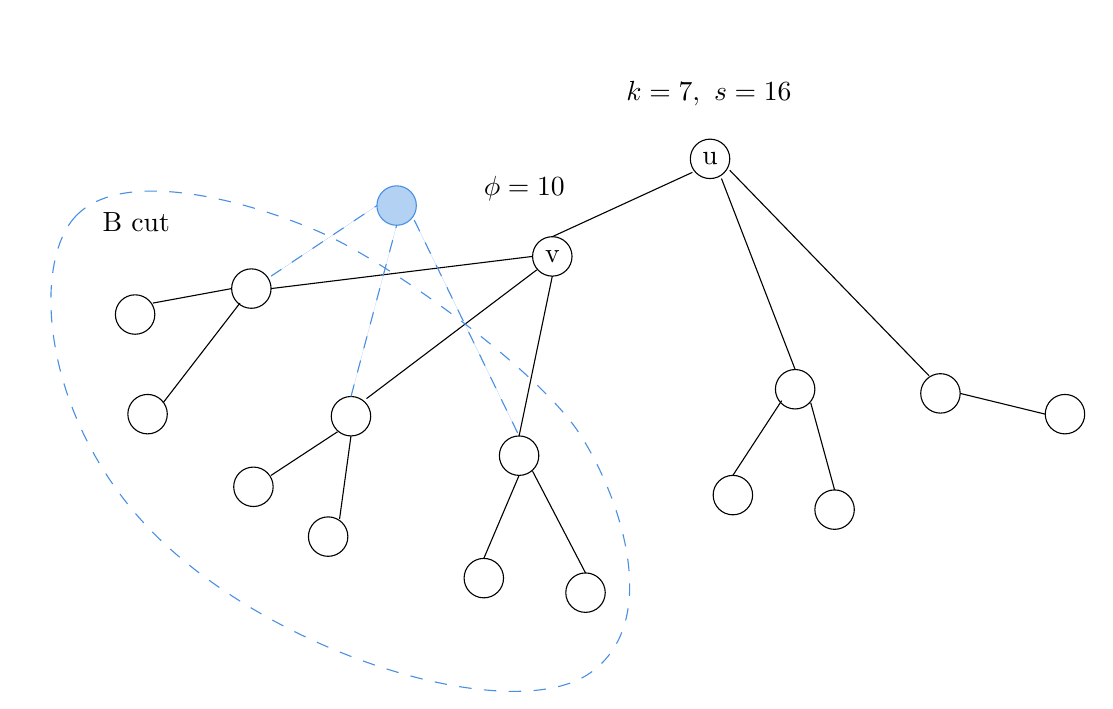
\begin{tikzpicture}[x=0.75pt,y=0.75pt,yscale=-1,xscale=1]
        %uncomment if require: \path (0,471); %set diagram left start at 0, and has height of 471

        %Shape: Circle [id:dp34076887970340053]
        \draw  [fill={rgb, 255:red, 255; green, 255; blue, 255 }  ,fill opacity=1 ] (392,61.5) .. controls (392,56.25) and (396.25,52) .. (401.5,52) .. controls (406.75,52) and (411,56.25) .. (411,61.5) .. controls (411,66.75) and (406.75,71) .. (401.5,71) .. controls (396.25,71) and (392,66.75) .. (392,61.5) -- cycle ;

        %Shape: Circle [id:dp9085081530378656]
        \draw  [fill={rgb, 255:red, 255; green, 255; blue, 255 }  ,fill opacity=1 ] (316,108.5) .. controls (316,103.25) and (320.25,99) .. (325.5,99) .. controls (330.75,99) and (335,103.25) .. (335,108.5) .. controls (335,113.75) and (330.75,118) .. (325.5,118) .. controls (320.25,118) and (316,113.75) .. (316,108.5) -- cycle ;

        %Shape: Circle [id:dp40613127689805917]
        \draw  [fill={rgb, 255:red, 255; green, 255; blue, 255 }  ,fill opacity=1 ] (403,223.5) .. controls (403,218.25) and (407.25,214) .. (412.5,214) .. controls (417.75,214) and (422,218.25) .. (422,223.5) .. controls (422,228.75) and (417.75,233) .. (412.5,233) .. controls (407.25,233) and (403,228.75) .. (403,223.5) -- cycle ;
        %Shape: Circle [id:dp9931876018636179]
        \draw  [fill={rgb, 255:red, 255; green, 255; blue, 255 }  ,fill opacity=1 ] (503,174.5) .. controls (503,169.25) and (507.25,165) .. (512.5,165) .. controls (517.75,165) and (522,169.25) .. (522,174.5) .. controls (522,179.75) and (517.75,184) .. (512.5,184) .. controls (507.25,184) and (503,179.75) .. (503,174.5) -- cycle ;
        %Shape: Circle [id:dp7698586857134941]
        \draw  [fill={rgb, 255:red, 255; green, 255; blue, 255 }  ,fill opacity=1 ] (563,184.5) .. controls (563,179.25) and (567.25,175) .. (572.5,175) .. controls (577.75,175) and (582,179.25) .. (582,184.5) .. controls (582,189.75) and (577.75,194) .. (572.5,194) .. controls (567.25,194) and (563,189.75) .. (563,184.5) -- cycle ;
        %Shape: Circle [id:dp07661905351809639]
        \draw  [fill={rgb, 255:red, 255; green, 255; blue, 255 }  ,fill opacity=1 ] (452,230.5) .. controls (452,225.25) and (456.25,221) .. (461.5,221) .. controls (466.75,221) and (471,225.25) .. (471,230.5) .. controls (471,235.75) and (466.75,240) .. (461.5,240) .. controls (456.25,240) and (452,235.75) .. (452,230.5) -- cycle ;
        %Shape: Circle [id:dp6823852359253104]
        \draw  [fill={rgb, 255:red, 255; green, 255; blue, 255 }  ,fill opacity=1 ] (433,172.5) .. controls (433,167.25) and (437.25,163) .. (442.5,163) .. controls (447.75,163) and (452,167.25) .. (452,172.5) .. controls (452,177.75) and (447.75,182) .. (442.5,182) .. controls (437.25,182) and (433,177.75) .. (433,172.5) -- cycle ;
        %Straight Lines [id:da2795330732074286]
        \draw    (407,71) -- (442.5,163) ;


        %Straight Lines [id:da95361289139327]
        \draw    (411,67) -- (507,166) ;


        %Straight Lines [id:da03919277897290474]
        \draw    (436,178) -- (412.5,214) ;


        %Straight Lines [id:da6790046753307697]
        \draw    (450,179) -- (461.5,221) ;


        %Straight Lines [id:da3674173158335614]
        \draw    (563,184.5) -- (522,174.5) ;


        %Straight Lines [id:da02933874590346841]
        \draw    (393,68) -- (325.5,99) ;


        %Shape: Circle [id:dp6930911043272474]
        \draw  [fill={rgb, 255:red, 255; green, 255; blue, 255 }  ,fill opacity=1 ] (172,219.5) .. controls (172,214.25) and (176.25,210) .. (181.5,210) .. controls (186.75,210) and (191,214.25) .. (191,219.5) .. controls (191,224.75) and (186.75,229) .. (181.5,229) .. controls (176.25,229) and (172,224.75) .. (172,219.5) -- cycle ;
        %Shape: Circle [id:dp4545176452788231]
        \draw  [fill={rgb, 255:red, 255; green, 255; blue, 255 }  ,fill opacity=1 ] (208,243.5) .. controls (208,238.25) and (212.25,234) .. (217.5,234) .. controls (222.75,234) and (227,238.25) .. (227,243.5) .. controls (227,248.75) and (222.75,253) .. (217.5,253) .. controls (212.25,253) and (208,248.75) .. (208,243.5) -- cycle ;
        %Shape: Circle [id:dp030374617759524325]
        \draw  [fill={rgb, 255:red, 255; green, 255; blue, 255 }  ,fill opacity=1 ] (219,185.5) .. controls (219,180.25) and (223.25,176) .. (228.5,176) .. controls (233.75,176) and (238,180.25) .. (238,185.5) .. controls (238,190.75) and (233.75,195) .. (228.5,195) .. controls (223.25,195) and (219,190.75) .. (219,185.5) -- cycle ;
        %Straight Lines [id:da016875084395338025]
        \draw    (222,193) -- (190,214) ;


        %Straight Lines [id:da7587321706433352]
        \draw    (228.5,195) -- (223,235) ;


        %Shape: Circle [id:dp6805190369347967]
        \draw  [fill={rgb, 255:red, 255; green, 255; blue, 255 }  ,fill opacity=1 ] (283,263.5) .. controls (283,258.25) and (287.25,254) .. (292.5,254) .. controls (297.75,254) and (302,258.25) .. (302,263.5) .. controls (302,268.75) and (297.75,273) .. (292.5,273) .. controls (287.25,273) and (283,268.75) .. (283,263.5) -- cycle ;
        %Shape: Circle [id:dp49294006336897334]
        \draw  [fill={rgb, 255:red, 255; green, 255; blue, 255 }  ,fill opacity=1 ] (332,270.5) .. controls (332,265.25) and (336.25,261) .. (341.5,261) .. controls (346.75,261) and (351,265.25) .. (351,270.5) .. controls (351,275.75) and (346.75,280) .. (341.5,280) .. controls (336.25,280) and (332,275.75) .. (332,270.5) -- cycle ;
        %Shape: Circle [id:dp4780933458297658]
        \draw  [fill={rgb, 255:red, 255; green, 255; blue, 255 }  ,fill opacity=1 ] (300,204.5) .. controls (300,199.25) and (304.25,195) .. (309.5,195) .. controls (314.75,195) and (319,199.25) .. (319,204.5) .. controls (319,209.75) and (314.75,214) .. (309.5,214) .. controls (304.25,214) and (300,209.75) .. (300,204.5) -- cycle ;
        %Straight Lines [id:da9579747847325664]
        \draw    (309.5,214) -- (292.5,254) ;


        %Straight Lines [id:da24682160488454663]
        \draw    (316,212) -- (341.5,261) ;


        %Straight Lines [id:da7254371683892009]
        \draw    (318,115) -- (236,177) ;


        %Straight Lines [id:da9361718285942648]
        \draw    (325.5,118) -- (309.5,195) ;


        %Shape: Circle [id:dp7136610740709559]
        \draw  [fill={rgb, 255:red, 255; green, 255; blue, 255 }  ,fill opacity=1 ] (171,124) .. controls (171,118.75) and (175.25,114.5) .. (180.5,114.5) .. controls (185.75,114.5) and (190,118.75) .. (190,124) .. controls (190,129.25) and (185.75,133.5) .. (180.5,133.5) .. controls (175.25,133.5) and (171,129.25) .. (171,124) -- cycle ;
        %Shape: Circle [id:dp7986023789770009]
        \draw  [fill={rgb, 255:red, 255; green, 255; blue, 255 }  ,fill opacity=1 ] (115,136.5) .. controls (115,131.25) and (119.25,127) .. (124.5,127) .. controls (129.75,127) and (134,131.25) .. (134,136.5) .. controls (134,141.75) and (129.75,146) .. (124.5,146) .. controls (119.25,146) and (115,141.75) .. (115,136.5) -- cycle ;
        %Straight Lines [id:da8486079993175883]
        \draw    (316,108.5) -- (190,124) ;


        %Straight Lines [id:da27547813733695325]
        \draw    (171,124) -- (133,131) ;


        %Shape: Circle [id:dp08981252883235546]
        \draw  [fill={rgb, 255:red, 255; green, 255; blue, 255 }  ,fill opacity=1 ] (121,184.5) .. controls (121,179.25) and (125.25,175) .. (130.5,175) .. controls (135.75,175) and (140,179.25) .. (140,184.5) .. controls (140,189.75) and (135.75,194) .. (130.5,194) .. controls (125.25,194) and (121,189.75) .. (121,184.5) -- cycle ;
        %Straight Lines [id:da22823959276419536]
        \draw    (175,131) -- (138,179) ;


        %Shape: Polygon Curved [id:ds15408437148876897]
        \draw  [color={rgb, 255:red, 74; green, 144; blue, 226 }  ,draw opacity=1 ][dash pattern={on 4.5pt off 4.5pt}] (96,89) .. controls (119,65) and (180,82) .. (214,97) .. controls (248,112) and (318,163) .. (338,193) .. controls (358,223) and (379,284) .. (344,309) .. controls (309,334) and (204,305) .. (142,250) .. controls (80,195) and (73,113) .. (96,89) -- cycle ;
        %Shape: Circle [id:dp5861650780323242]
        \draw  [color={rgb, 255:red, 74; green, 144; blue, 226 }  ,draw opacity=1 ][fill={rgb, 255:red, 179; green, 209; blue, 243 }  ,fill opacity=1 ] (241,84) .. controls (241,78.75) and (245.25,74.5) .. (250.5,74.5) .. controls (255.75,74.5) and (260,78.75) .. (260,84) .. controls (260,89.25) and (255.75,93.5) .. (250.5,93.5) .. controls (245.25,93.5) and (241,89.25) .. (241,84) -- cycle ;
        %Straight Lines [id:da880896354333569]
        \draw [color={rgb, 255:red, 74; green, 144; blue, 226 }  ,draw opacity=1 ][fill={rgb, 255:red, 74; green, 144; blue, 226 }  ,fill opacity=1 ] [dash pattern={on 4.5pt off 4.5pt}]  (190,118) -- (241,84) ;


        %Straight Lines [id:da2721999945811009]
        \draw [color={rgb, 255:red, 74; green, 144; blue, 226 }  ,draw opacity=1 ][fill={rgb, 255:red, 74; green, 144; blue, 226 }  ,fill opacity=1 ] [dash pattern={on 4.5pt off 4.5pt}]  (228.5,176) -- (250.5,93.5) ;


        %Straight Lines [id:da9627189828730469]
        \draw [color={rgb, 255:red, 74; green, 144; blue, 226 }  ,draw opacity=1 ][fill={rgb, 255:red, 74; green, 144; blue, 226 }  ,fill opacity=1 ] [dash pattern={on 4.5pt off 4.5pt}]  (259,91) -- (309.5,195) ;



        % Text Node
        \draw (401.5,61.5) node  [align=left] {u};
        % Text Node
        \draw (325.5,108.5) node  [align=left] {v};
        % Text Node
        \draw (312,76) node  [align=left] {$\displaystyle \phi =10$};
        % Text Node
        \draw (401,30) node [color={rgb, 255:red, 0; green, 0; blue, 0 }  ,opacity=1 ] [align=left] {$\displaystyle k=7,\ s=16$};
        % Text Node
        \draw (125,92) node  [align=left] {B cut};


    \end{tikzpicture}

    \caption{Example decompose step}\label{fig:decompose_example}
\end{figure}

The component size is \(s=16\), and the anonymization parameter is \(k=7\). \(s \ge \max \{ 2k-1,3k-5\} = \max \{ 13, 16 \} \) is true, so the component is considered oversized and needs to be cut.
The root of the largest sized subtree is \textit{v}, and its size is \(\phi=10\).

Since \(s-\phi \ge k-1\), we can proceed with one of the cut types.
In fact, in this case \(s-\phi=k-1=6\), so we will need to apply cut type B as highlighted by the dotted line in figure~\ref{fig:decompose_example}.

In order to keep the nodes in the cut partition together, we insert a \emph{Steiner's Vertex}.
This vertex is also highlighted on figure~\ref{fig:decompose_example} with dotted edges.

The resulting two partitions are of size 7 and 9 --- note, that the \emph{Steiner's Vertex} does not count into the component's size.
Both partitions are of proper size now.

\subsection{Polynomial-time approximation algorithm}\label{subsec:polynomial-time-approximation-algorithm}

\paragraph{Theorem}  There is a polynomial-time algorithm for the k-Anonymity problem, that achieves an approximation ratio of \(\max \{ 2k-1, 3k-5 \} \)~\cite{aggarwal}.

\paragraph{Proof} First, use algorithm \textsc{Forest} to create a forest with cost at most OPT and minimum tree size at least \textit{k}.
Then repeatedly apply algorithm \textsc{Decompose component} to any component that has size larger than \(\max \{ 2k-1, 3k-5 \} \).
Note that both these algorithms terminate in \(\mathcal{O}(kn^2)\) time~\cite{aggarwal}.

\section{Summary}
In this chapter we have briefly introduced the Go programming language, and why we think it is a good choice for implementing the anonymization algorithm.

Then we took a high-level overview of the algorithm implementation, including the different pieces, and how they work together. After which we discussed in what format the algorithm will accept the input data. We gave a detailed description of how generalization works, and how one can use the built-in generalizers or implement a custom one.

Next we justified our decision on the selected graph library used by the program, and went through the most important steps of the  graph algorithm one-by-one: cost graph calculation, forest building and decomposition.

Then we have shown a code listing for a full run of the anonymizer program for a small sample data table, and illustrated a possible result. Finally we briefly looked at how the continuous mode works for the anonymizer, and when we can take advantage of it.

In the next chapter we will talk about testing, performance and benchmarks.

\chapter{Implementation in Go}\label{ch:chapter_implementation}
\section{Overview}

\subsection{Why Go?}

\emph{Go} (also known as \emph{Golang}) is a relatively new programming language. It first appeared in 2009 and has gained a tremendous amount of popularity in the recent few years. \cite{wiki08} The language itself is a compiled, statically typed general purpose systems programming language. It is similar to C in many ways, but with memory safety, garbage collection and structural typing.

But why has it gained such popularity? The language itself is very small and easy to learn. Its features are pragmatic and carefully selected to fix problems with other mainstream languages. It encourages readability


\subsection{Development}

\subsection{Hosting}

\subsection{Structure}

\subsection{Graph representation}

\subsection{Importing the library}

\section{Public API}

\subsection{Providing the input table}

\subsection{Providing the generalizers}

\subsubsection{Hierarchy generalizers}

\subsubsection{Custom generalizers}

\section{Core algorithm}

\subsection{Cost graph building}

\subsection{Forest building}

\subsection{Decomposition}

\section{Wrapping it up}

\chapter{Tests, Benchmarks}\label{ch:chapter_tests}
\section{Testing in Go}\label{sec:testing-in-go}
\begin{figure}[H]
    \centering
    \small
    \begin{tabular}{r l}
        \toprule
        Number of unit tests added          & 126 \\
        Number of integration tests added   & 18 \\
        Test coverage increase (models)     & 100\% \\
        Test coverage increase (BLL)        & 45\% \\
        \bottomrule
    \end{tabular}
    \caption{Testing the anonymization framework}\label{fig:tests_added}
\end{figure}

\section{Algorithm Correctness}\label{sec:correctness}
In this section we will reason about the \emph{correctness of the implementation}.

We will be relying on the unit and integration test suite that has been created along with the algorithm.
It should be noted, that unit tests alone will not give a \emph{mathematical} proof of correctness, or total correctness (the former proves input-output correctness, while the latter also includes proof of termination). However, with a well-tested codebase we can almost certainly tell with a \emph{high degree of confidence}, that the code performs according to the specifications.

\subsection{Generalizer tests}

For each built-in generalizer implementation a corresponding test suite verifies the correct behavior. Without getting too much into the details, Figure~\ref{fig:generalizer_tests} shows a summary of the tests and their locations.

\vspace{\baselineskip}
\begin{figure}[H]
    \centering
    \small
    \begin{tabular}{r p{8cm}}
        \toprule
        \textbf{File} & \textbf{Functionality} \\
        \midrule
        \texttt{suppressor\_test.go}               & verifies basic suppression functionality \\
        \texttt{hierarchy\_test.go}                & basic \& auto builder, including edge cases for non-full trees and invalid input \\
        \texttt{hierarchy\_generalizer\_test.go}   & generalization to different levels, and related edge cases, benchmarks \\
        \texttt{range\_generalizer\_test.go}       & tests for int \& float ranges, including range validation, virtual hierarchy splitting and levels \\
        \texttt{prefix\_generalizer\_test.go}      & tests the prefix generalization logic, including validation of input \\
        \bottomrule
    \end{tabular}
    \caption{Generalizer Tests}\label{fig:generalizer_tests}
\end{figure}

\subsection{Core algorithm tests}

\subsubsection{Cost graph tests}
These tests cover the building and edge-cost calculation of cost graphs. The test suite in \texttt{cost\_test.go} deals with verifying the cost calculation formula. Another test suite verifies that the  cost-graph is built properly. In these tests the input is always a \emph{table}, and we verify, that the structure and edge-costs of the output graph is as expected. Tests also cover edge cases, like invalid data in the table, invalid generalizer for the column and empty input. The cost graph test suite is located in \texttt{cost\_graph\_test.go}.

\subsubsection{Forest building tests}
The tests for the forest building algorithm are located in \texttt{anon\_graph\_test.go}, and they verify the following aspects of the algorithm:
\begin{itemize}
    \setstretch{1.0}
    \item a correct component should be picked for extension
    \item a correct vertex should be picked as source vertex
    \item a correct vertex should be picked as target vertex
    \item forest (tree) properties are not violated after the new edge is added
\end{itemize}

\subsubsection{Decompose tests}
The decompose step is a rather complex step in the core algorithm. The test suite in the file \texttt{decompose\_test.go} tries to deal with this complexity. With the proper set of helper methods however, the tests in it are still readable and relatively easy to follow. An example can be seen on Figure~\ref{lst:decompose_test}.

Tests in the decompose suite are centered around the verification of the following:
\begin{itemize}
    \setstretch{1.0}
    \item oversized threshold calculation logic
    \item component picked for decomposition is actually oversized
    \item cut types A through D (see Section~\ref{subsec:algorithm-to-decompose-oversized-components})
    \item handling of Steiner's vertices
    \item the algorithm stops when there are no more oversized components in the forest
\end{itemize}

\begin{lstlisting}[caption=A test for Decompose Cut type B,label=lst:decompose_test,float,floatplacement=H]
//            ------- 0 ------
//           |                |
//      ---- 1 ----           6
//     |     |     |          |
//     2     3     4          7
//           |
//           5
//
//  u := 0, v := 1, k := 4, s > 2k-1
//  s-t == k-1
func TestPartition_TypeBCut(t *testing.T) {
    g := GetUndirectedTestGraph2()
    d := NewDecomposer(g, 4)
    u := g.Node(0)
    v := g.Node(1)
    d.performCutTypeB(u, v)
    testutil.AssertVertexReplaced(t, g, 1, 8, 2, 3, 4)
}
\end{lstlisting}

\subsubsection{Anonoymizer tests}
Last, but not least the tests in \texttt{anonymize\_test.go} check, that all the above work well together. They call the \texttt{Anonymizer} for a set of test input tables, and verify that \emph{k-anonymity} on the output is not violated. This is done by ensuring, that in the resulting output for any given row at least \(k-1\) other rows must be the same partition. (See Listing~\ref{lst:test_k_anonymity}.)

\begin{lstlisting}[caption=Asserting k-anonymity,label=lst:test_k_anonymity,float,floatplacement=H]
func assertKAnonymity(table *model.Table, k int, t *testing.T) {
    for i, r1 := range table.GetRows() {
        count := 0
        for _, r2 := range table.GetRows() {
            if inSamePartition(r1, r2, table.GetSchema()) {
                count++
            }
        }
        if count < k {
            t.Errorf("K-anonymity violated in row %v", i)
        }
    }
}
\end{lstlisting}

\subsection{Examples}
Several of the above tests also have \emph{testable examples}. Examples in Go are special tests, which contain a runnable snippet of code, that demonstrates API usage or functionality. They will be run by the testing framework along with the rest of the tests, and their example output will be verified automatically. A mismatch in the example output will cause the test to fail.

Each provided testable example is listed on Figure~\ref{fig:testable_examples}.

\vspace{\baselineskip}
\begin{figure}[H]
    \centering
    \small
    \begin{tabular}{r p{8cm}}
        \toprule
        \textbf{File} & \textbf{Functionality} \\
        \midrule
        \texttt{anonymize\_example.go}   & demonstrates basic anonymization \\
        \texttt{continuous\_example.go}  & demonstrates continuous anonymization \\
        \bottomrule
    \end{tabular}
    \caption{Testable examples}\label{fig:testable_examples}
\end{figure}

\subsection{Stats \& metrics}
Table~\ref{fig:test_metrics} shows some interesting metrics about the project.

\vspace{\baselineskip}
\begin{figure}[H]
    \centering
    \small
    \begin{tabular}{r c}
        \toprule
        \textbf{Metric} & \textbf{Value} \\
        \midrule
        Total LOC                      & 4370 \\
        Number of source files         & 44 \\
        Number of test source files    & 21 \\
        Number of Unit Tests           & 257 \\
        Number of Benchmarks           & 12 \\
        Number of Examples             & 2 \\
        Statement Coverage             & 90.5\% \\
        \bottomrule
    \end{tabular}
    \caption{Metrics}\label{fig:test_metrics}
\end{figure}

\section{Performance, Benchmarks}\label{sec:benchmarks}
In this section we will present the results of the benchmarks executed on the anonymization algorithm, and compare the results to the expected algorithm characteristics introduced earlier in Chapter~\ref{ch:chapter_algorithm}. As mentioned in Section~\ref{subsec:benchmarks} benchmarks in Go are special tests, which can be executed with the testing framework. Go will help us run the analyzed function until the measure is \emph{stable}, and is able to precisely calculate the average execution time.

\subsection{Test Rig}

The configuration that was used for executing the benchmarks is summarized on Figure~\ref{fig:test_rig}.
\begin{figure}[H]
    \centering
    \small
    \begin{tabular}{r l}
        \toprule
        Operating System Kernel        & Linux 5.3.1-arch \\
        CPU Model                      & Intel® Pentium® G4620 @ 3.70GHz \\
        CPU Cores                      & 2 \\
        Total Memory                   & 16335268 kB \\
        Go Version                     & go1.13 linux/amd64 \\
        Anonymizer Version             & 1.2.7 \\
        \bottomrule
    \end{tabular}
    \caption{Benchmark test rig}\label{fig:test_rig}
\end{figure}

\subsection{RangeGeneralizer benchmarks}

Figure~\ref{fig:range_bm} shows a comparison benchmark of both range based generalizers --- \texttt{IntRange} and \texttt{FloatRange}. The horizontal axis plots the size of the range (note the logarithmic scale), the vertical axis shows the \emph{average time to generalize the median value in the range to the highest level} in nanoseconds as measured by the Go bench framework. As expected, both show a linear progression curve. Generalizing float ranges is much more expensive however, this is due to the increased number of splits and additional cost of comparison with delta.

\vspace{\baselineskip}
\begin{figure}[ht]
    \centering
    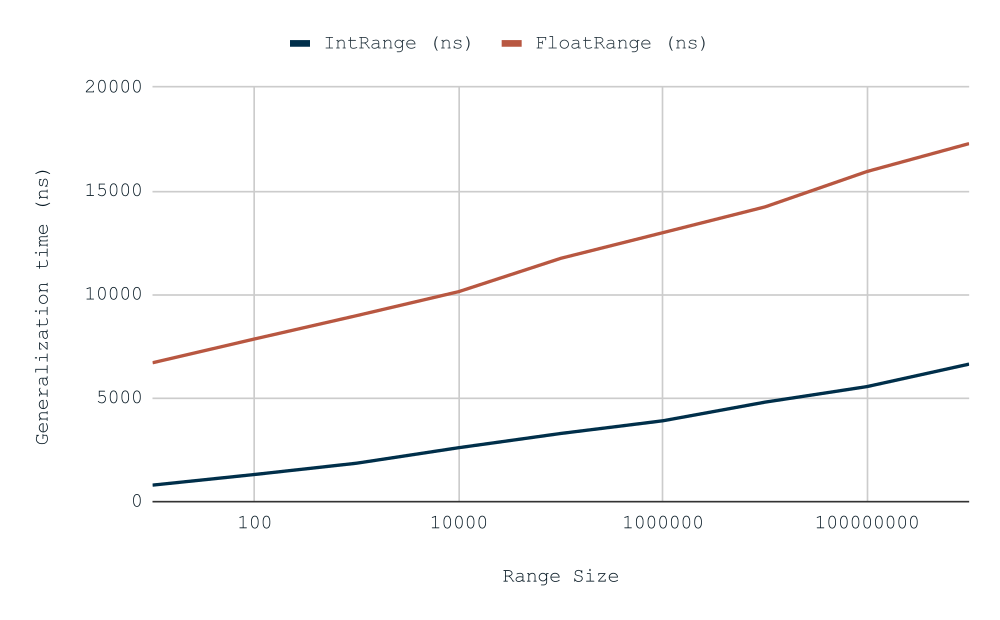
\includegraphics[width=0.8\textwidth]{images/range.png}
    \caption{Range Generalizer Benchmarks}\label{fig:range_bm}
\end{figure}

\subsection{PrefixGeneralizer benchmarks}

The \texttt{PrefixGeneralizer} has three different parameters. For each benchmark, we will test one parameter while the other two are fixed. The tests always generalize the input to the \emph{maximum possible level}.

\subsubsection{Word Count}

In this test we set the maximum allowed words to a high enough fixed value, and benchmark the performance based on the \emph{actual number of words} (amount of text) on the input of the generalizer. Figure~\ref{fig:prefix_word_count_bm} shows a relatively flat exponential curve. The performance starts to degrade after 5000 words, which is an indicator of the amount of (English) text it is supposed to be able to handle per cell in the input data table.

\vspace{\baselineskip}
\begin{figure}[H]
    \centering
    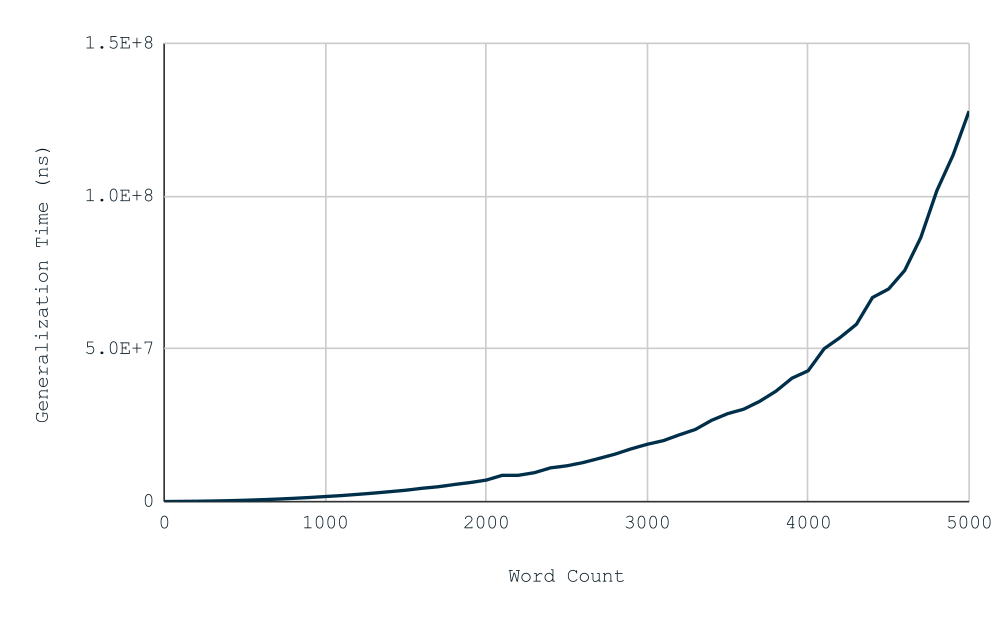
\includegraphics[width=0.8\textwidth]{images/prefix-word-count.png}
    \caption{Prefix --- Word Count Benchmark}\label{fig:prefix_word_count_bm}
\end{figure}

\subsubsection{Word Length}

As discussed during the introduction of the prefix generalizer in Section~\ref{subsec:prefix_generalizer} the performance of the prefix generalization algorithm should be \emph{unaffected} by the length of words. The benchmark on Figure~\ref{fig:prefix_word_length_bm} proves this adequately. The time needed to generalize with fixed max words, word count and increasing word length assumes a flat line.

\vspace{\baselineskip}
\begin{figure}[H]
    \centering
    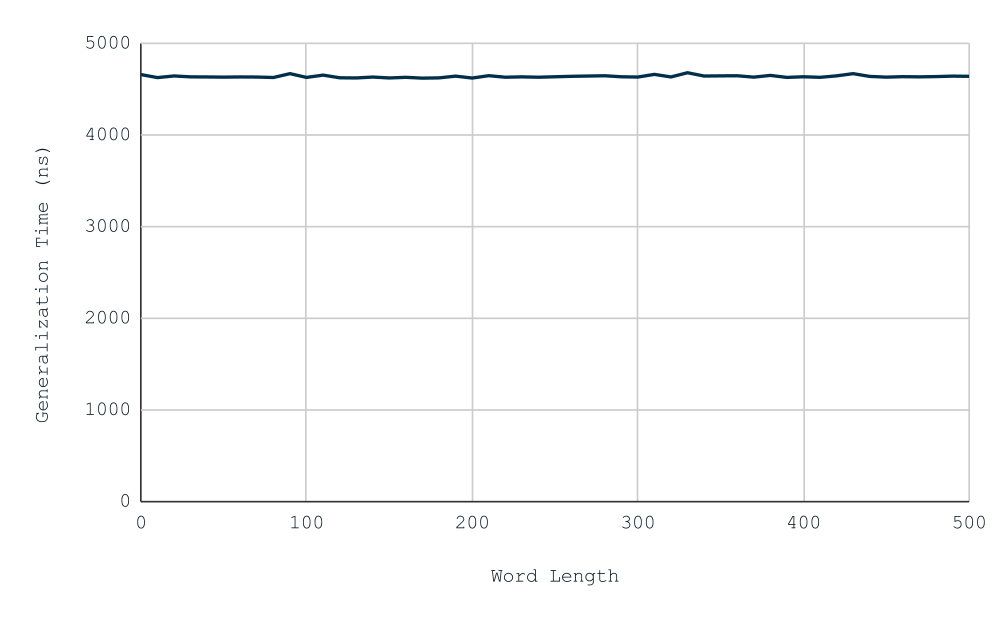
\includegraphics[width=0.8\textwidth]{prefix-word-length.png}
    \caption{Prefix --- Word Length Benchmark}\label{fig:prefix_word_length_bm}
\end{figure}

\subsubsection{Max Words}

Finally we inspect the effect of the \texttt{MaxWords} parameter. We can recall, that this parameter increases the \emph{total levels} of the generalizer, even when the actual number of words in the generalized text is smaller. Thus the linear curve visible on Figure~\ref{fig:prefix_max_words_bm} seems realistic.

\vspace{\baselineskip}
\begin{figure}[H]
    \centering
    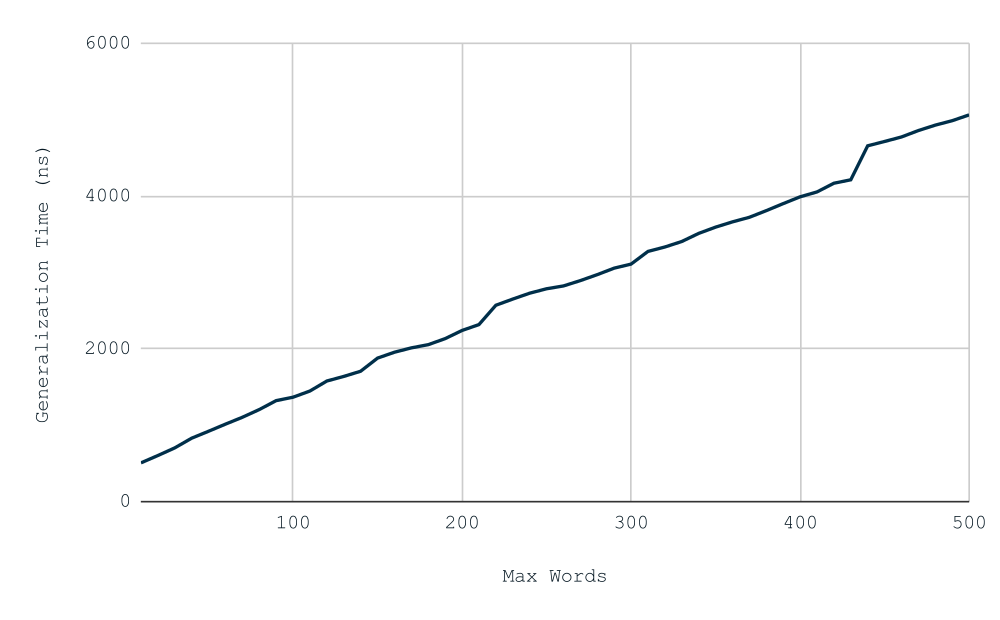
\includegraphics[width=0.8\textwidth]{images/prefix-max-words.png}
    \caption{Prefix --- Max Words Benchmark}\label{fig:prefix_max_words_bm}
\end{figure}

\subsection{HierarchyGeneralizer benchmarks}

\subsubsection{Hierarchy depth}
One way hierarchies can be benchmarked is based on their depth. Given a fixed node count, the number of levels correlates to the number of children each node in the hierarchy has. Since it is easier to build a hierarchy by specifying the number of children per node, we will use this approach for our benchmark. Figure~\ref{fig:hierarchy_children_bm} shows an interesting result (note the logarithmic vertical axis). The generalization time greatly improves with a more flat hierarchy up to around 4 or 5 children. Increasing the child-count further has no significant beneficial effect. The explanation for this behavior is, that while the generalization hierarchy is not actually a search-tree, increasing the child-count thus reducing the total number of levels for the same amount of nodes will actually improve the number of steps needed to locate the partition a given item belongs to on a certain level (up to a certain threshold).
\vspace{\baselineskip}
\begin{figure}[H]
    \centering
    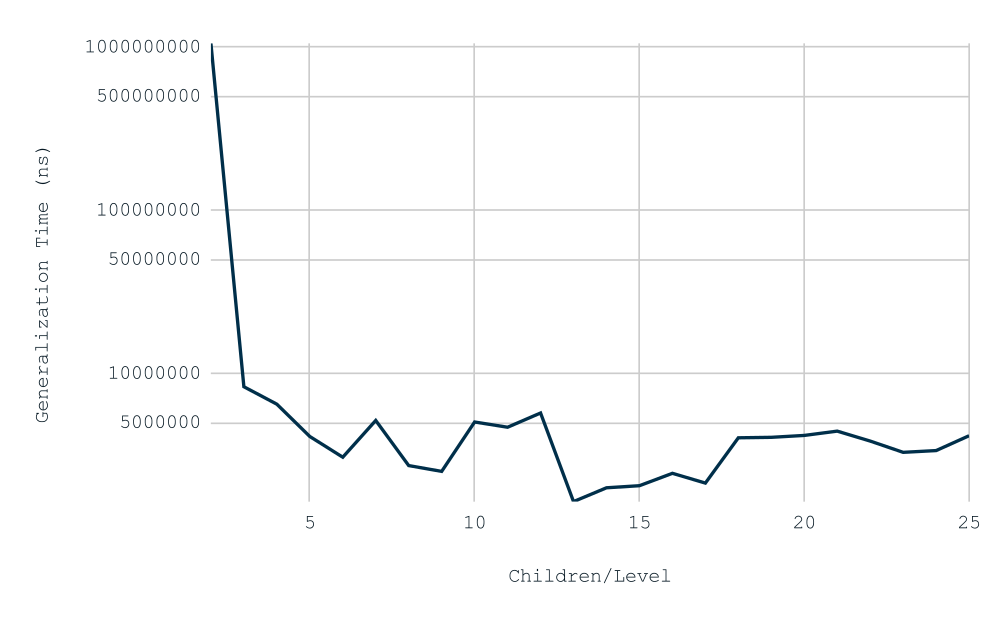
\includegraphics[width=0.8\textwidth]{hierarchy-children.png}
    \caption{Hierarchy --- Children per Node Benchmark}\label{fig:hierarchy_children_bm}
\end{figure}

\subsubsection{Number of nodes}
By increasing the number of nodes in the hierarchy, the generalization time will increase in a linear fashion as shown on Figure~\ref{fig:hierarchy_nodes_bm}.
\vspace{\baselineskip}
\begin{figure}[H]
    \centering
    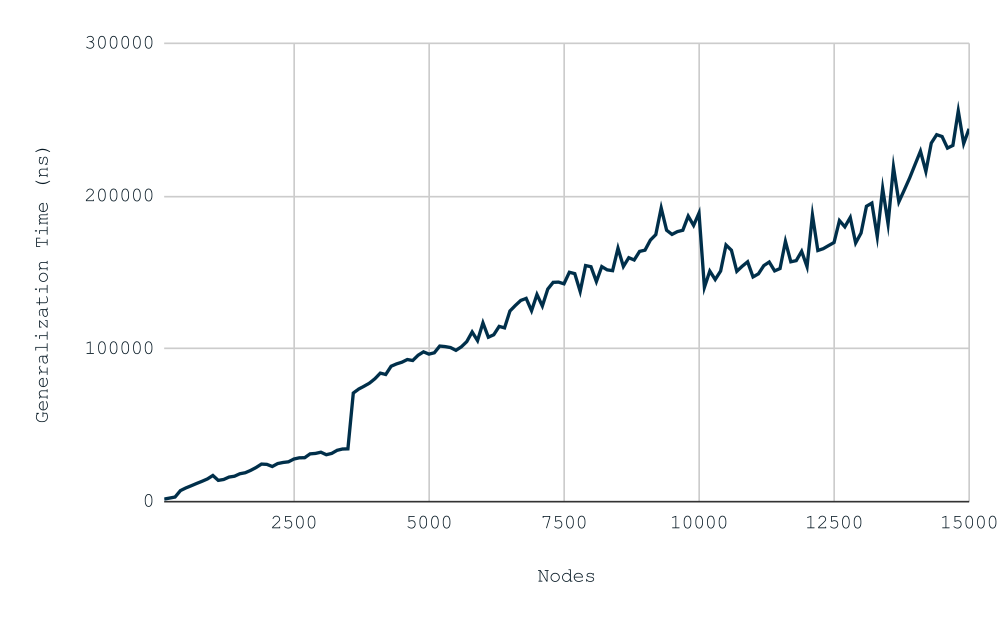
\includegraphics[width=0.8\textwidth]{images/hierarchy-nodes.png}
    \caption{Hierarchy --- Number of Nodes Benchmark}\label{fig:hierarchy_nodes_bm}
\end{figure}

\subsection{Comparison of generalizers}

Plotting all the built-in generalizers on the same chart gives a good opportunity to compare their relative performance. Note, that each generalizer has various parameters which affect the performance greatly, so the following comparisons are only approximate guidelines.

According to Figure~\ref{fig:compare_all} the slowest generalizer is the \texttt{FloatRange} generalizer. In order to get a better overview, Figure~\ref{fig:compare_fast} shows the same setup with \texttt{FloatRange} omitted.

\vspace{\baselineskip}
\begin{figure}[ht]
    \centering
    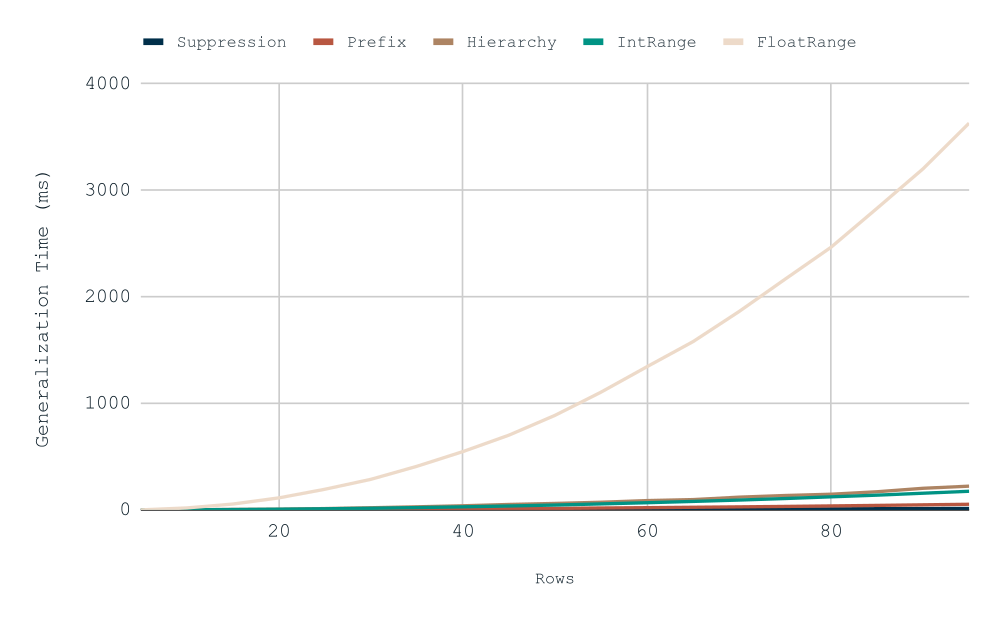
\includegraphics[width=0.8\textwidth]{images/compare-all.png}
    \caption{Generalizer Speed Comparison}\label{fig:compare_all}
\end{figure}

\vspace{\baselineskip}
\begin{figure}[H]
    \centering
    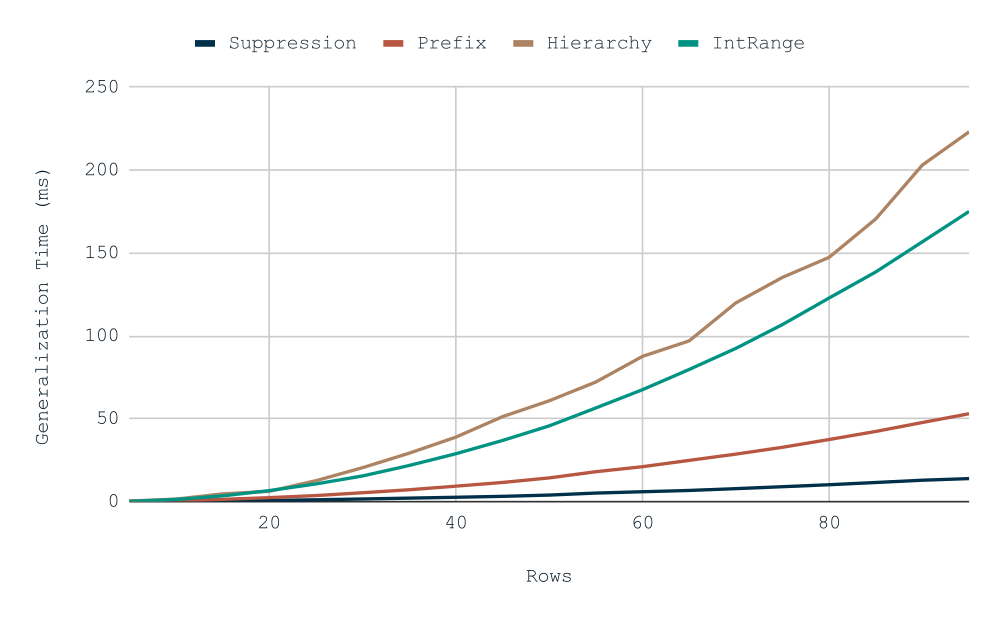
\includegraphics[width=0.8\textwidth]{images/compare-fast.png}
    \caption{Generalizer Speed Comparison (without FloatRange)}\label{fig:compare_fast}
\end{figure}

\subsection{Anonymization benchmarks}

The following benchmarks measure the anonymization of a full sample data table. The table contains only integer numbers generalized with the same \texttt{IntRange} generalizer. The benchmark variables are the \emph{column count}, the \emph{row count} and the \emph{k} anonymity parameter.

\subsubsection{Column count}

We can expect the generalization time to increase for increasing the number of columns in the table. The reason is, that we need to compare more data when calculating the \emph{scaled generalization cost} for the cost-graph. This extra amount of work however is only linear, as shown on Figure~\ref{fig:anon_columns}.

\vspace{\baselineskip}
\begin{figure}[H]
    \centering
    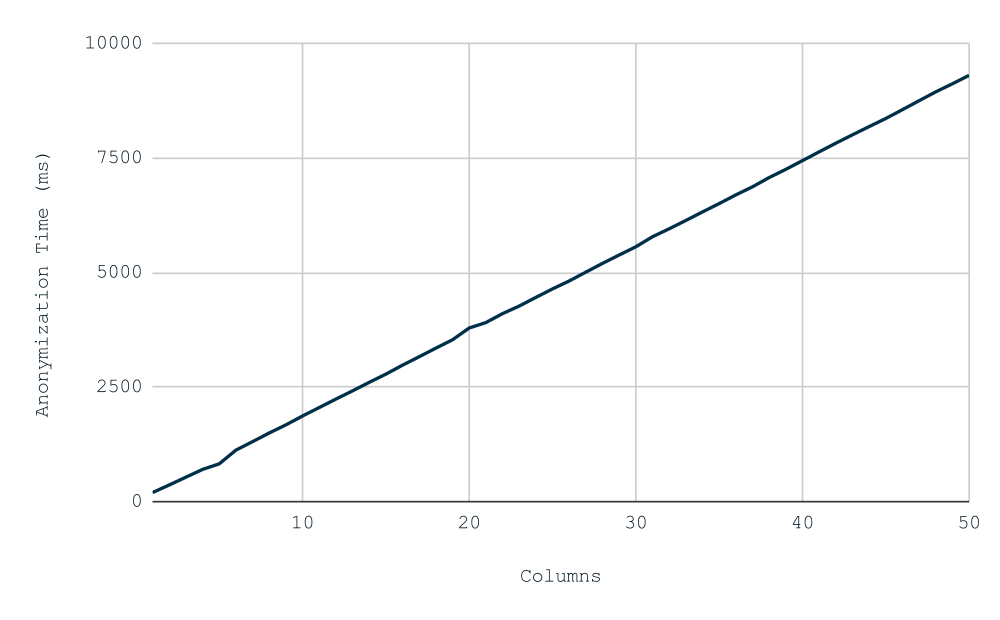
\includegraphics[width=0.8\textwidth]{anon-columns.png}
    \caption{Anonymization vs Column count}\label{fig:anon_columns}
\end{figure}

\subsubsection{Row count}

This is the most important benchmark of all of the above, as it (indirectly) measures the core implementation of the graph based approximation algorithm. As proven in Section~\ref{subsec:polynomial-time-approximation-algorithm} increasing the number of rows in the table should result in a \(\mathcal{O}(kn^2)\) curve. The benchmark on Figure~\ref{fig:anon_rows} confirms, that our implementation of the algorithm has the same characteristics.

\vspace{\baselineskip}
\begin{figure}[ht]
    \centering
    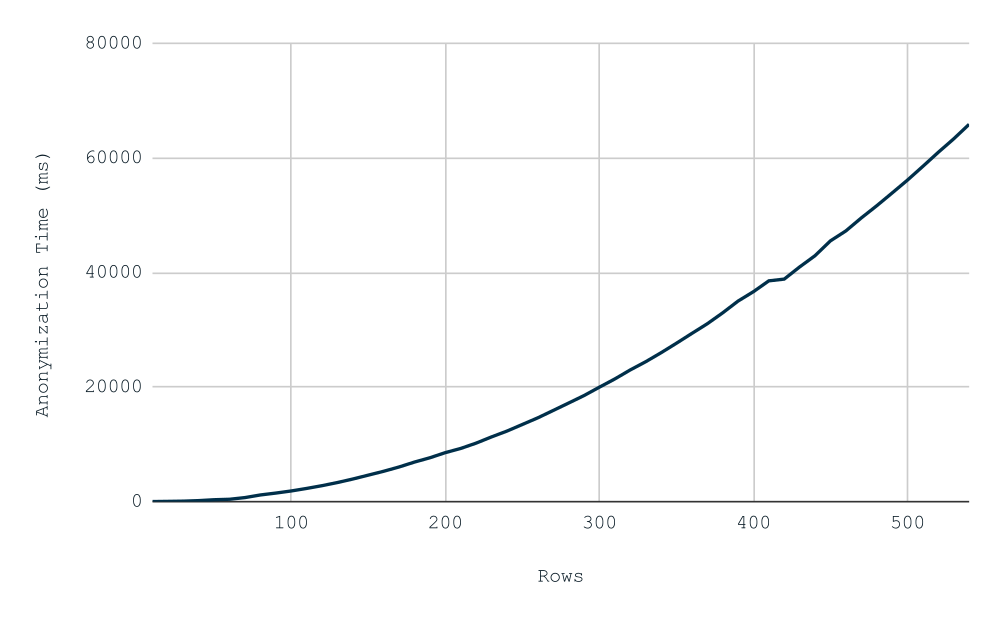
\includegraphics[width=0.8\textwidth]{anon-rows.png}
    \caption{Anonymization vs Row count}\label{fig:anon_rows}
\end{figure}

\subsubsection{k value}

Finally, we investigate if the \emph{k} anonymity parameter has any effect on the anonymization time. In this benchmark the \emph{k} value was increased from 2 to 100 while having all other input parameters fixed. The only restriction is, that the data table needs to contain at least \emph{k} number of rows in order to be able to achieve k-anonymity. The resulting benchmark can be seen on Figure~\ref{fig:anon_k} and shows, that the \emph{k} value has no measurable effect on the anonymization time for a static sized input table.

\vspace{\baselineskip}
\begin{figure}[ht]
    \centering
    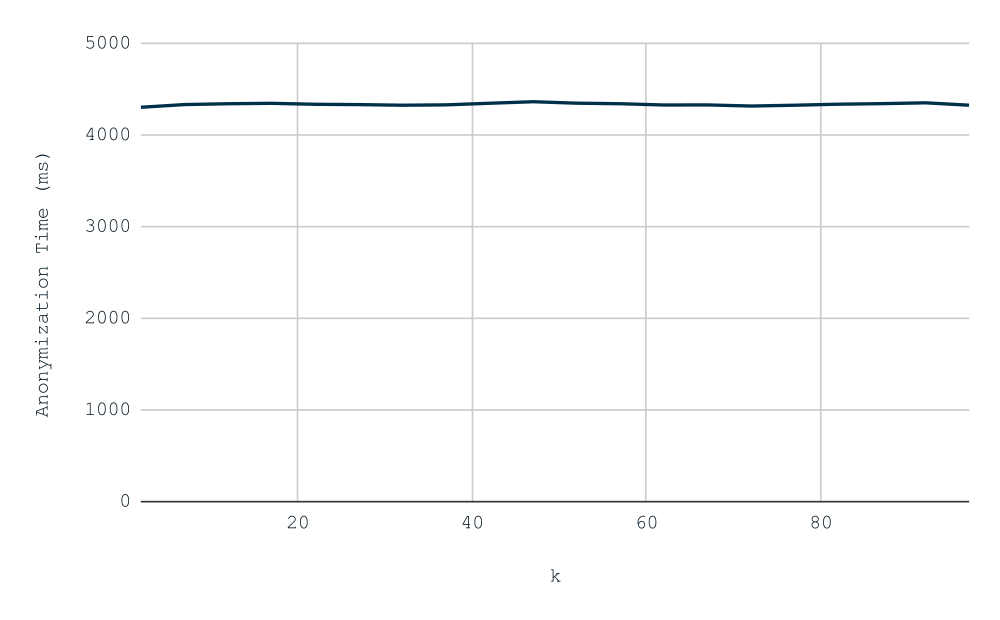
\includegraphics[width=0.8\textwidth]{images/anon-k.png}
    \caption{Anonymization  time vs the \emph{k} anonymity parameter}\label{fig:anon_k}
\end{figure}

\chapter{Integration}\label{ch:chapter_integration}
\section{Importing the library}\label{sec:importing_the_library}
\subsection{Library location}
The library is published as a \emph{Go module} to a well-known source control provider using \emph{git}. Instructions on usage, and the full source code are available on the project's home page~\cite{k-anon}. A developer intending to use the library has several options to start using it:
\begin{enumerate}
    \setstretch{1.0}
    \item add a direct dependency using Go modules \emph{(recommended)}
    \item use the \texttt{`go get'} command to download it to the \texttt{\$GOPATH}
    \item clone the source code and build it manually
\end{enumerate}

\subsection{Go modules}

\subsubsection{Adding module dependencies}

Go added support for managing direct and indirect dependencies starting from version \textit{1.11}. The implementation is based on \textit{v-go}. Direct and indirect dependencies are managed in a \texttt{go.mod} file located at the root of the project. When an import to an external module is declared in a source file, Go will automatically obtain \emph{latest} stable version of the module and it's dependencies when building the project --- this is done automatically, and normally there is no need to interact with the \texttt{go.mod} file directly. However, if needed the \texttt{`go get'} and \texttt{`go mod'} commands can be used to manage go modules explicitly (sync, upgrade, etc.).

For example, to start using the graph anonymization library with Go modules, one would add the import on Listing~\ref{lst:go_import}. Go will automatically obtain the latest stable version of the library and register the dependency in the \texttt{go.mod} file (see Listing~\ref{lst:go_mod}).

\begin{lstlisting}[caption=Importing the graph library,label=lst:go_import,float,floatplacement=H]
import "bitbucket.org/dargzero/k-anon"
\end{lstlisting}


\begin{lstlisting}[caption=The \texttt{go.mod} file,label=lst:go_mod,float,floatplacement=H]
require (
    bitbucket.org/dargzero/k-anon v1.2.6
    gonum.org/v1/netlib v0.0.0-20190327185612-36a5df7c87e8 // indirect
    // ...
)
\end{lstlisting}


\subsubsection{Publishing modules}

In order to \emph{publish} a Go project as a module, it needs to be under supported source control. This is usually git, but Mercurial, Bazaar and others are also supported~\cite{publish-go-modules}. Once the project repository is hosted, new releases can be created by \emph{tagging} a commit with a version using \emph{semantic versioning}. A go module's semantic version has the form of \texttt{vMAJOR.MINOR.PATH}. (Semantic versioning itself will not be discussed in this document.)

For example, for the graph anonymization library a few tagged versions can be seen on Figure~\ref{fig:tagged_versions}.
\begin{figure}[H]
    \centering
    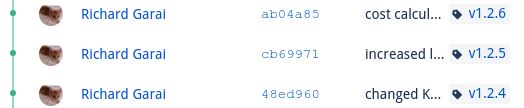
\includegraphics[width=0.8\textwidth]{images/tagged-versions.png}
    \caption{Tagged versions}\label{fig:tagged_versions}
\end{figure}

\section{Integration Case Study}\label{sec:integration_example}
In this section we will give a detailed walk-through of an integration case study. We will show how to use the graph anonymization library in an existing Go code base. This existing code base is a containerized anonymization system leveraging the MongoDb document database. It was developed by \emph{Vilmos Sz. Martinek} as part of his MSc thesis while studying at \textit{Budapest University of Technology and Economics} in 2018~\cite{martinek}. A cornerstone of the integration is to make the \emph{minimum amount of changes} in the existing system, while introducing an alternative anonymization algorithm as an optionally selectable component.

\subsection{Overview of the target system}

The target anonymization system implements a standard three-tiered architecture. See Figure~\ref{fig:integration_arch}. We highlighted network boundaries with blue dashed lines on the figure.

\subsubsection{REST API}\label{subsubsec:rest_api}
Client applications can use the system through a provided REST API, which supports two operations: \emph{data set creation} and \emph{data upload}. The former makes it possible to push data into different MongoDb collections, the latter deals with actually receiving the data in the form of JSON documents.

\vspace{\baselineskip}
\begin{figure}[H]
    \centering


\tikzset{every picture/.style={line width=0.75pt}} %set default line width to 0.75pt

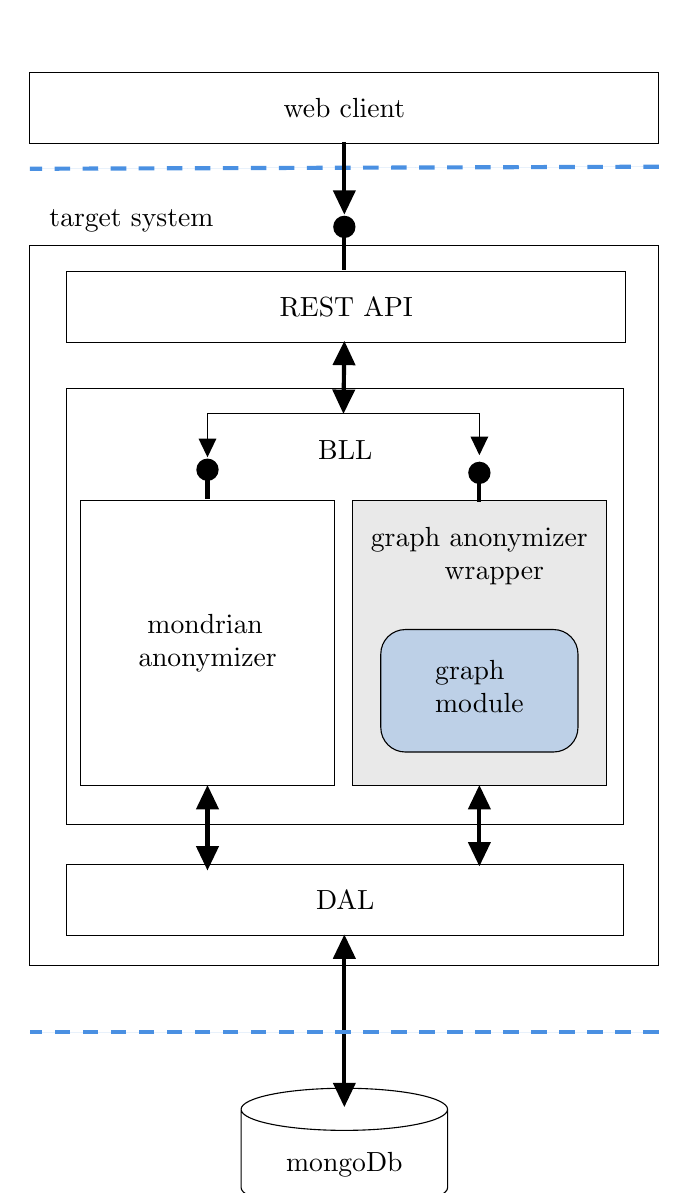
\begin{tikzpicture}[x=0.75pt,y=0.75pt,yscale=-1,xscale=1]
%uncomment if require: \path (0,571); %set diagram left start at 0, and has height of 571

%Shape: Rectangle [id:dp25314219983411235]
\draw  [fill={rgb, 255:red, 155; green, 155; blue, 155 }  ,fill opacity=0.22 ] (349.75,216) -- (472.25,216) -- (472.25,353) -- (349.75,353) -- cycle ;
%Rounded Rect [id:dp6104192131332256]
\draw  [fill={rgb, 255:red, 74; green, 144; blue, 226 }  ,fill opacity=0.28 ] (363.5,289.8) .. controls (363.5,283.28) and (368.78,278) .. (375.3,278) -- (446.7,278) .. controls (453.22,278) and (458.5,283.28) .. (458.5,289.8) -- (458.5,325.2) .. controls (458.5,331.72) and (453.22,337) .. (446.7,337) -- (375.3,337) .. controls (368.78,337) and (363.5,331.72) .. (363.5,325.2) -- cycle ;
%Shape: Rectangle [id:dp7542396041522255]
\draw   (194.38,9.62) -- (497.5,9.62) -- (497.5,43.63) -- (194.38,43.63) -- cycle ;

%Shape: Rectangle [id:dp8775304827751447]
\draw   (194.37,93) -- (497.5,93) -- (497.5,440) -- (194.37,440) -- cycle ;
%Shape: Rectangle [id:dp29329734503174665]
\draw   (212.25,105.63) -- (481.5,105.63) -- (481.5,139.63) -- (212.25,139.63) -- cycle ;

%Shape: Rectangle [id:dp3924156131636001]
\draw   (212.25,162) -- (480.5,162) -- (480.5,372) -- (212.25,372) -- cycle ;
%Shape: Rectangle [id:dp02053336225786917]
\draw   (212.25,391.41) -- (480.5,391.41) -- (480.5,425.41) -- (212.25,425.41) -- cycle ;

%Shape: Rectangle [id:dp8663149504803358]
\draw   (218.75,216) -- (341.25,216) -- (341.25,353) -- (218.75,353) -- cycle ;
%Flowchart: Magnetic Disk [id:dp36269861006508]
\draw   (395.69,509.15) -- (395.69,546.85) .. controls (395.69,552.46) and (373.41,557) .. (345.94,557) .. controls (318.46,557) and (296.19,552.46) .. (296.19,546.85) -- (296.19,509.15)(395.69,509.15) .. controls (395.69,514.76) and (373.41,519.3) .. (345.94,519.3) .. controls (318.46,519.3) and (296.19,514.76) .. (296.19,509.15) .. controls (296.19,503.54) and (318.46,499) .. (345.94,499) .. controls (373.41,499) and (395.69,503.54) .. (395.69,509.15) -- cycle ;

%Straight Lines [id:da08877933566463603]
\draw [color={rgb, 255:red, 74; green, 144; blue, 226 }  ,draw opacity=1 ][fill={rgb, 255:red, 74; green, 144; blue, 226 }  ,fill opacity=1 ][line width=1.5]  [dash pattern={on 5.63pt off 4.5pt}]  (497.5,55) -- (194.38,56) ;


%Straight Lines [id:da5932184702081]
\draw [line width=1.5]    (345.94,84) -- (345.94,105) ;

\draw [shift={(345.94,84)}, rotate = 90] [color={rgb, 255:red, 0; green, 0; blue, 0 }  ][fill={rgb, 255:red, 0; green, 0; blue, 0 }  ][line width=1.5]      (0, 0) circle [x radius= 4.36, y radius= 4.36]   ;
%Straight Lines [id:da8662427461600262]
\draw [line width=1.5]    (345.94,43) -- (345.94,75) ;
\draw [shift={(345.94,78)}, rotate = 270] [fill={rgb, 255:red, 0; green, 0; blue, 0 }  ][line width=1.5]  [draw opacity=0] (11.61,-5.58) -- (0,0) -- (11.61,5.58) -- cycle    ;

%Straight Lines [id:da5790521830826718]
\draw [line width=1.5]    (345.94,428) -- (345.94,505) ;
\draw [shift={(345.94,508)}, rotate = 270] [fill={rgb, 255:red, 0; green, 0; blue, 0 }  ][line width=1.5]  [draw opacity=0] (11.61,-5.58) -- (0,0) -- (11.61,5.58) -- cycle    ;
\draw [shift={(345.94,425)}, rotate = 90] [fill={rgb, 255:red, 0; green, 0; blue, 0 }  ][line width=1.5]  [draw opacity=0] (11.61,-5.58) -- (0,0) -- (11.61,5.58) -- cycle    ;
%Straight Lines [id:da9813732944058937]
\draw [line width=1.5]    (345.9,142) -- (345.54,171) ;
\draw [shift={(345.5,174)}, rotate = 270.72] [fill={rgb, 255:red, 0; green, 0; blue, 0 }  ][line width=1.5]  [draw opacity=0] (11.61,-5.58) -- (0,0) -- (11.61,5.58) -- cycle    ;
\draw [shift={(345.94,139)}, rotate = 90.72] [fill={rgb, 255:red, 0; green, 0; blue, 0 }  ][line width=1.5]  [draw opacity=0] (11.61,-5.58) -- (0,0) -- (11.61,5.58) -- cycle    ;
%Straight Lines [id:da5100456793816999]
\draw [line width=1.5]    (280,356) -- (280,391) ;
\draw [shift={(280,394)}, rotate = 270] [fill={rgb, 255:red, 0; green, 0; blue, 0 }  ][line width=1.5]  [draw opacity=0] (11.61,-5.58) -- (0,0) -- (11.61,5.58) -- cycle    ;
\draw [shift={(280,353)}, rotate = 90] [fill={rgb, 255:red, 0; green, 0; blue, 0 }  ][line width=1.5]  [draw opacity=0] (11.61,-5.58) -- (0,0) -- (11.61,5.58) -- cycle    ;
%Straight Lines [id:da9511987307073959]
\draw [color={rgb, 255:red, 74; green, 144; blue, 226 }  ,draw opacity=1 ][fill={rgb, 255:red, 74; green, 144; blue, 226 }  ,fill opacity=1 ][line width=1.5]  [dash pattern={on 5.63pt off 4.5pt}]  (497.5,472) -- (194.37,472) ;


%Straight Lines [id:da6634746570080241]
\draw [line width=1.5]    (280,201) -- (280,215) ;

\draw [shift={(280,201)}, rotate = 90] [color={rgb, 255:red, 0; green, 0; blue, 0 }  ][fill={rgb, 255:red, 0; green, 0; blue, 0 }  ][line width=1.5]      (0, 0) circle [x radius= 4.36, y radius= 4.36]   ;
%Straight Lines [id:da11396993553443457]
\draw [line width=1.5]    (411,202.5) -- (411,216.5) ;

\draw [shift={(411,202.5)}, rotate = 90] [color={rgb, 255:red, 0; green, 0; blue, 0 }  ][fill={rgb, 255:red, 0; green, 0; blue, 0 }  ][line width=1.5]      (0, 0) circle [x radius= 4.36, y radius= 4.36]   ;
%Straight Lines [id:da6497437274365285]
\draw [line width=1.5]    (411,356) -- (411,389) ;
\draw [shift={(411,392)}, rotate = 270] [fill={rgb, 255:red, 0; green, 0; blue, 0 }  ][line width=1.5]  [draw opacity=0] (11.61,-5.58) -- (0,0) -- (11.61,5.58) -- cycle    ;
\draw [shift={(411,353)}, rotate = 90] [fill={rgb, 255:red, 0; green, 0; blue, 0 }  ][line width=1.5]  [draw opacity=0] (11.61,-5.58) -- (0,0) -- (11.61,5.58) -- cycle    ;
%Straight Lines [id:da30407000837324416]
\draw    (280,193) -- (280,174) -- (411,174) -- (411,192) ;
\draw [shift={(411,194)}, rotate = 270] [fill={rgb, 255:red, 0; green, 0; blue, 0 }  ][line width=0.75]  [draw opacity=0] (8.93,-4.29) -- (0,0) -- (8.93,4.29) -- cycle    ;
\draw [shift={(280,195)}, rotate = 270] [fill={rgb, 255:red, 0; green, 0; blue, 0 }  ][line width=0.75]  [draw opacity=0] (8.93,-4.29) -- (0,0) -- (8.93,4.29) -- cycle    ;

% Text Node
\draw (411,305.5) node [scale=1] [align=left] { graph\\module};
% Text Node
\draw (243.38,81.25) node  [align=left] {target system};
% Text Node
\draw (346.88,122.63) node  [align=left] {REST API};
% Text Node
\draw (346.37,408.41) node  [align=left] {DAL};
% Text Node
\draw (346.38,191.63) node  [align=left] {BLL};
% Text Node
\draw (280,284.5) node  [align=left] { \ mondrian\\anonymizer};
% Text Node
\draw (411,242.63) node  [align=left] {graph anonymizer\\ \ \ \ \ \ \ \ \ wrapper};
% Text Node
\draw (345.94,536) node  [align=left] {mongoDb};
% Text Node
\draw (345.94,26.63) node  [align=left] {web client};


\end{tikzpicture}
    \caption{Integration with the target system}\label{fig:integration_arch}
\end{figure}

\subsubsection{BLL}
The business logic layer contains the anonymization related code. This is where we need to implement the integration with the graph based anonymizer. Initially the system supported a single anonymization algorithm, called \emph{Mondrian}. Mondrian is a top-down greedy anonymization algorithm, which uses a \emph{kd-tree} to partition the raw data into partitions for generalization. In this document we will not discuss the Mondrian algorithm in further details --- we can simply think about it as another anonymization algorithm with different characteristics than the graph based anonymizer. In certain circumstances it might be beneficial to use one versus the other, so it would be useful to be able to switch between the two types of algorithms for different data sets.

The BLL layer already contained an interface which encapsulates the public API of an anonymizer, hence the need for a \emph{wrapper} around the graph anonymizer. The wrapper provides a thin layer around the API introduced in Section~\ref{sec:example_run} and makes it compatible with the rest of the system.

\subsubsection{DAL}
The data access layer uses the \emph{mgo} third party library to interface with MongoDb. Since this layer is not the focus point for our integration case study, we will not detail its internals in this document.

\subsection{Adapting the input data format}\label{subsec:json_input_format}
As mentioned in~\ref{subsubsec:rest_api}, both the configuration and upload of the data is done through the REST API, so our first step will be to extend the input declaration, and make it able to switch between algorithms and configure parameters for both types of algorithms.

\paragraph{Original input format:} an example of the unmodified input format can be seen on Listing~\ref{lst:original_format}. The structure contains a \textit{settings} and \textit{fields} object. The former describes the anonymization parameters, the latter the field definitions (or \emph{schema}). Each field can have:
\begin{itemize}
    \setstretch{1.0}
    \item \textbf{name:} the name of the column
    \item \textbf{mode:} how the column should be treated. Can be \textit{id} or \textit{qid}
    \item \textbf{type:} data type for anonymization. Can be \textit{numeric}, \textit{prefix}
\end{itemize}

\vspace{\baselineskip}
\begin{lstlisting}[caption=Original input format,label=lst:original_format,float,floatplacement=H]
{
  "settings": {
    "k": 3,
    "algorithm": "mondrian",
    "mode": "single"
  },
  "fields": [
    {
      "name": "name",
      "mode": "qid",
      "type": "prefix"
    },
    //...
}
\end{lstlisting}


\paragraph{Modified input format:} fortunately the \textit{settings} object already supports defining the algorithm name (even though initially only the Mondrian value was supported), so this field can be reused. We can also reuse most of the field settings as well, however we need to introduce a couple of extra data types and also make it possible to configure the generalizers when selecting the graph anonymizer.

\vspace{\baselineskip}
\begin{lstlisting}[caption=Modified input format,label=lst:modified_format,float,floatplacement=H]
{
    "settings": {
        "k": 3,
        "algorithm": "graph",
        "mode": "single"
    },
    "fields": [
        {
            "name": "name",
            "mode": "drop"
        },
        {
            "name": "age",
            "mode": "qid",
            "type": "numeric",
            "opts": {
                "type": "int",
                "min": 0,
                "max": 150
            }
        },
        {
            "name": "salary",
            "mode": "qid",
            "type": "numeric",
            "opts": {
                "type": "float",
                "min": 0,
                "max": 200000
            }
        },
        {
            "name": "motto",
            "mode": "qid",
            "type": "prefix",
            "opts": {
                "max": 150
            }
        }
    ]
}
\end{lstlisting}



The modified input format is shown on Listing~\ref{lst:modified_format}. We now allow the \textit{``graph''} value for the \textit{algorithm} field. We also introduced the \textit{``keep''} and \textit{``drop''} values for the \textit{mode} field to be able to have a finer control over what columns to anonymize, leave alone, or suppress completely.

The field configuration objects now allow an \textit{``opts''} object. This will only be processed by the graph wrapper, the Mondrian module will ignore it entirely. This object contains graph anonymizer related parameters for certain field types (\textit{min}, \textit{max} values for range generalizers, and a \textit{max}-words setting for prefix generalizers).

\subsection{Implementing the wrapper}

The framework provides the \texttt{anonymizerAlgorithm} interface as an abstraction for the top level API of anonymization. Mondrian is an implementation of this interface, and we will need to implement the wrapper to be an implementation as well. Figure~\ref{lst:anon_interface} shows the interface.

\vspace{\baselineskip}
\begin{lstlisting}[caption=The \texttt{anonymizerAlgorithm interfcae},label=lst:anon_interface,float,floatplacement=H]
type anonymizerAlgorithm interface {
	initialize(*anonmodel.Dataset, string, []anonmodel.FieldAnonymizationInfo)
	anonymize() error
}
\end{lstlisting}

The \texttt{initialize} method is called by the framework after instantiating the anonymizer, but before calling the \texttt{anonymize} method. It gets the parsed settings for the fields and data set from the input JSON detailed in~\ref{subsec:json_input_format}. We can use this method to initialize the schema, since the modified JSON input now contains all the required information to declare the columns with the appropriate generalizer for each field. Note, that the actual data to anonymize is not passed to the wrapper by the framework (see~\ref{subsec:anonymizing_the_data}).

\subsection{Anonymizing the data}\label{subsec:anonymizing_the_data}

Recall from~\ref{subsubsec:rest_api}, that the client facing interface provided a separate web method for \emph{uploading data}. It is the responsibility of the implementor of \texttt{anonymizerAlgorithm} to get hold of the data for the data set specified in the parameters. In essence, the graph wrapper will need to have a reference to the DAL, and when the \texttt{anonymize} method is called by the framework, it must first query the data waiting to be anonymized. When the anonymization is finished, it should insert the anonymized data and mark it \emph{done}.

\subsection{Tests}

Finally, after the wrapper has been implemented, we needed to verify that the modified system is working correctly. The following types of testing have been performed:
\begin{itemize}
    \setstretch{1.0}
    \item \textbf{unit tests:} in these tests we need to mock the data access layer, and verify that input parsing, schema declaration and anonymization is working correctly.
    \item \textbf{regression:} normally we run the framework-provided unit test suite to verify, that we did not break any existing functionality. Unfortunately there were no unit tests in the original code base. This leaves us with the only option to first \emph{before touching anything} cover the most important parts of the original code base (for the original functionality) with tests, until a sufficient coverage rate is reached. \emph{Then} proceed with implementing our changes, where we can verify by running the test suite at any time that our added functionality is not breaking existing features. Before actually modifying the existing code base, I have taken a great care to cover as much of the original functionality as possible (see Figure~\ref{fig:tests_added}).
    \item \textbf{integration tests:} we verify, that integration between the BLL \& REST API, and BLL \& MongoDb isn't broken. We can do this by bringing up the system in the provided \emph{docker} container and calling the REST API with an HTTP client, or checking the data queried/inserted from/to the database respectively.
\end{itemize}

\vspace{\baselineskip}
\begin{figure}[H]
    \centering
    \small
    \begin{tabular}{r l}
        \toprule
        Number of unit tests added          & 126 \\
        Number of integration tests added   & 18 \\
        Test coverage increase (models)     & 100\% \\
        Test coverage increase (BLL)        & 45\% \\
        \bottomrule
    \end{tabular}
    \caption{Testing the anonymization framework}\label{fig:tests_added}
\end{figure}

\chapter{Improvements, Future Work}\label{ch:chapter_future_work}
\section{Improved algorithm}

The original work on which our graph algorithm implementation is based on presents an improved algorithm for the \(k=2\) and \(k=3\) special cases~\cite{aggarwal}. If the use case often requires the use of \(k=2\) or \(k=3\) anonymity, it might be beneficial to extend the anonymizer to handle these special cases differently.

\subsection{Improved algorithm for k=2}\label{subsec:improved_algorithm}
The method presented in Section~\ref{ch:chapter_algorithm} gives a \textit{3-approximation} algorithm for the \(k=2\) case. However, there is a polynomial time \textit{1.5-approximation} algorithm when \(k=2\) and using a \textit{binary alphabet}. Note, that for a binary alphabet generalization is equivalent to suppression~\cite{aggarwal}.

This special algorithm creates the cost-graph by considering the \textit{Hamming distance} between the vectors represented by two nodes in the graph. Then we obtain a \textbf{minimum-weight} \([1,2]\)-factor \textit{F} of \textit{G}.

\paragraph{Definition} A \([1,2]\)-factor of an edge-weighted graph \textit{G} is defined to be a spanning sub-graph \textit{F} of \textit{G} such that each vertex in \textit{F} has a degree of 1 or 2~\cite{aggarwal}.

It has been shown, that finding a minimum-weight \([1,2]\)-factor of a graph can be computed in polynomial time (Cornuejols, 1988).

We treat each component in the obtained \textit{F} graph as a \textit{cluster}, and retain the bits where they agree on each vector, and suppress them otherwise.

\paragraph{Theorem} the number of \texttt{*}s introduced by the above algorithm is at most \(1.5\) times the number of \texttt{*}s in an \textit{optimal} 2-anonymity solution~\cite{aggarwal}.

\subsection{Improved algorithm for k=3}

Also for a binary alphabet, it is possible to give a \textit{2-approximation} algorithm for the \(k=3\) case~\cite{aggarwal}. This algorithm uses a similar algorithm to~\ref{subsec:improved_algorithm}, with the exception of now calculating \textbf{minimum-weight} 2-factor \textit{F} spanning sub-graph, which can also be done in polynomial time.

\paragraph{Theorem} the resulting 2-factor \textit{F} can be transformed into a 2-approximation solution for 3-anonymity~\cite{aggarwal}.


\section{Performance}

The result of the performance benchmarks in~\ref{sec:benchmarks} shows, that the \textit{FloatRangeGeneralizer} and \textit{HierarchyGeneralizer} in particular suffer from poor performance, especially when the respective range size and node count is larger. To a smaller extent, the same problem can be observed with the \textit{PrefixGeneralizer} when the word count is more than 5000 words.

Improving the performance of these generalizers might be possible by reducing the step count needed to locate an item among the possible list of partitions on a given level. It might also be possible to introduce a better data structure for the generalizers that can eliminate the need to scan through all partitions on each level, thus reducing search step count significantly for larger input.

\appendix
\chapter{Appendix}\label{ch:chapter_appendix}
\section{Raw benchmark data}

\subsection{Range Generalizer}
\vspace{\baselineskip}
\begin{figure}[H]
    \centering
    \footnotesize
    \begin{tabular}{r r r}
        \toprule
        \textbf{Range Size}      & \textbf{IntRange (ns)}      & \textbf{FloatRange (ns)} \\
        \midrule
        10              & 795   & 6704  \\
        100	            & 1309  & 7853  \\
        1000            & 1854  & 8980  \\
        10000	        & 2603	& 10138 \\
        100000	        & 3290	& 11747 \\
        1000000	        & 3902	& 12985 \\
        10000000	    & 4801	& 14228 \\
        100000000	    & 5553	& 15938 \\
        1000000000	    & 6638	& 17285 \\
        \bottomrule
    \end{tabular}
    \caption{Range Generalizer Benchmarks}
\end{figure}

\subsection{Prefix Generalizer}
\vspace{\baselineskip}
\begin{figure}[H]
    \centering
    \footnotesize
    \begin{tabular}{r r r}
        \toprule
        \textbf{word count} & \textbf{ns} \\
        \midrule
        0 & 30 \\
        100 & 59546 \\
        200 & 105497 \\
        300 & 183211 \\
        400 & 289844 \\
        500 & 427525 \\
        600 & 605834 \\
        700 & 806579 \\
        800 & 1052435 \\
        900 & 1326327 \\
        1000 & 1648000 \\
        1100 & 1965540 \\
        1200 & 2358381 \\
        1300 & 2771751 \\
        1400 & 3238024 \\
        1500 & 3712466 \\
        1600 & 4347377 \\
        1700 & 4844343 \\
        1800 & 5577968 \\
        1900 & 6227003 \\
        2000 & 7035743 \\
        2100 & 8602095 \\
        2200 & 8604262 \\
        2300 & 9468134 \\
        2400 & 11044884 \\
        2500 & 11706140 \\
        2600 & 12753449 \\
        2700 & 14114183 \\
        2800 & 15528353 \\
        2900 & 17257878 \\
        3000 & 18756047 \\
        3100 & 19943107 \\
        3200 & 21854827 \\
        3300 & 23629397 \\
        3400 & 26601383 \\
        3500 & 28787468 \\
        3600 & 30251983 \\
        3700 & 32855990 \\
        3800 & 36138043 \\
        3900 & 40409367 \\
        4000 & 42825120 \\
        4100 & 50063026 \\
        4200 & 53768189 \\
        4300 & 58040075 \\
        4400 & 66816700 \\
        4500 & 69603857 \\
        4600 & 75672948 \\
        4700 & 86444390 \\
        4800 & 101823757 \\
        4900 & 113373991 \\
        5000 & 127829247 \\
        \bottomrule
    \end{tabular}
    \quad
    \begin{tabular}{r r r}
        \toprule
        \textbf{word length} & \textbf{ns} \\
        \midrule
        0 & 4660 \\
        10 & 4627 \\
        20 & 4645 \\
        30 & 4635 \\
        40 & 4634 \\
        50 & 4632 \\
        60 & 4634 \\
        70 & 4633 \\
        80 & 4628 \\
        90 & 4670 \\
        100 & 4629 \\
        110 & 4654 \\
        120 & 4625 \\
        130 & 4623 \\
        140 & 4633 \\
        150 & 4623 \\
        160 & 4630 \\
        170 & 4621 \\
        180 & 4624 \\
        190 & 4643 \\
        200 & 4622 \\
        210 & 4648 \\
        220 & 4631 \\
        230 & 4635 \\
        240 & 4631 \\
        250 & 4636 \\
        260 & 4641 \\
        270 & 4644 \\
        280 & 4647 \\
        290 & 4636 \\
        300 & 4633 \\
        310 & 4662 \\
        320 & 4634 \\
        330 & 4680 \\
        340 & 4644 \\
        350 & 4646 \\
        360 & 4647 \\
        370 & 4632 \\
        380 & 4651 \\
        390 & 4629 \\
        400 & 4636 \\
        410 & 4630 \\
        420 & 4646 \\
        430 & 4670 \\
        440 & 4640 \\
        450 & 4632 \\
        460 & 4637 \\
        470 & 4635 \\
        480 & 4638 \\
        490 & 4643 \\
        500 & 4641 \\
        \bottomrule
    \end{tabular}
    \quad
    \begin{tabular}{r r r}
        \toprule
        \textbf{maxWords} & \textbf{ns} \\
        \midrule
        0 & --- \\
        10 & 507 \\
        20 & 603 \\
        30 & 703 \\
        40 & 830 \\
        50 & 921 \\
        60 & 1014 \\
        70 & 1104 \\
        80 & 1205 \\
        90 & 1322 \\
        100 & 1367 \\
        110 & 1448 \\
        120 & 1579 \\
        130 & 1639 \\
        140 & 1707 \\
        150 & 1879 \\
        160 & 1956 \\
        170 & 2013 \\
        180 & 2055 \\
        190 & 2134 \\
        200 & 2241 \\
        210 & 2318 \\
        220 & 2571 \\
        230 & 2652 \\
        240 & 2729 \\
        250 & 2787 \\
        260 & 2824 \\
        270 & 2894 \\
        280 & 2972 \\
        290 & 3057 \\
        300 & 3110 \\
        310 & 3276 \\
        320 & 3334 \\
        330 & 3406 \\
        340 & 3512 \\
        350 & 3594 \\
        360 & 3663 \\
        370 & 3723 \\
        380 & 3810 \\
        390 & 3902 \\
        400 & 3991 \\
        410 & 4055 \\
        420 & 4169 \\
        430 & 4214 \\
        440 & 4659 \\
        450 & 4716 \\
        460 & 4775 \\
        470 & 4859 \\
        480 & 4930 \\
        490 & 4988 \\
        500 & 5064 \\
        \bottomrule
    \end{tabular}
    \caption{Prefix Generalizer Benchmarks}
\end{figure}

\subsection{Hierarchy Generalizer}
\vspace{\baselineskip}
\begin{figure}[H]
    \centering
    \footnotesize
    \begin{tabular}{r r r}
        \toprule
        \textbf{children} & \textbf{ns} \\
        \midrule
        2 & 1056879442 \\
        3 & 8315230 \\
        4 & 6500438 \\
        5 & 4120536 \\
        6 & 3076307 \\
        7 & 5167282 \\
        8 & 2733832 \\
        9 & 2518081 \\
        10 & 5055884 \\
        11 & 4696178 \\
        12 & 5741875 \\
        13 & 1644598 \\
        14 & 1998117 \\
        15 & 2057829 \\
        16 & 2450867 \\
        17 & 2135154 \\
        18 & 4045385 \\
        19 & 4072653 \\
        20 & 4182987 \\
        21 & 4444684 \\
        22 & 3862781 \\
        23 & 3295126 \\
        24 & 3378286 \\
        25 & 4165054 \\
        \bottomrule
    \end{tabular}
    \quad
    \begin{tabular}{r r r}
        \toprule
        \textbf{nodes} & \textbf{ns} \\
        \midrule
        100 & 1662 \\
        200 & 2305 \\
        300 & 2976 \\
        400 & 7207 \\
        500 & 8935 \\
        600 & 10374 \\
        700 & 11874 \\
        800 & 13296 \\
        900 & 14835 \\
        1000 & 17098 \\
        1100 & 13891 \\
        1200 & 14474 \\
        1300 & 16059 \\
        1400 & 16606 \\
        1500 & 18225 \\
        1600 & 18892 \\
        1700 & 20441 \\
        1800 & 22309 \\
        1900 & 24564 \\
        2000 & 24365 \\
        2100 & 22966 \\
        2200 & 24890 \\
        2300 & 25615 \\
        2400 & 26046 \\
        2500 & 27871 \\
        2600 & 28653 \\
        2700 & 28734 \\
        2800 & 31244 \\
        2900 & 31538 \\
        3000 & 32328 \\
        3100 & 30692 \\
        3200 & 31543 \\
        3300 & 33572 \\
        3400 & 34417 \\
        3500 & 34527 \\
        3600 & 71080 \\
        3700 & 73695 \\
        3800 & 75560 \\
        3900 & 77584 \\
        4000 & 80440 \\
        4100 & 84116 \\
        4200 & 83214 \\
        4300 & 88625 \\
        4400 & 90148 \\
        4500 & 91264 \\
        4600 & 93014 \\
        4700 & 92378 \\
        4800 & 95833 \\
        4900 & 98041 \\
        5000 & 96559 \\
        \bottomrule
    \end{tabular}
    \quad
    \begin{tabular}{r r r}
        \toprule
        \textbf{nodes} & \textbf{ns} \\
        \midrule
        5100 & 97433 \\
        5200 & 101836 \\
        5300 & 101486 \\
        5400 & 100850 \\
        5500 & 99034 \\
        5600 & 101323 \\
        5700 & 104722 \\
        5800 & 111060 \\
        5900 & 105415 \\
        6000 & 117037 \\
        6100 & 107633 \\
        6200 & 109224 \\
        6300 & 114716 \\
        6400 & 113749 \\
        6500 & 124802 \\
        6600 & 128412 \\
        6700 & 131704 \\
        6800 & 133044 \\
        6900 & 124982 \\
        7000 & 135592 \\
        7100 & 128056 \\
        7200 & 139121 \\
        7300 & 143559 \\
        7400 & 143703 \\
        7500 & 142592 \\
        7600 & 150160 \\
        7700 & 149253 \\
        7800 & 137579 \\
        7900 & 154540 \\
        8000 & 153790 \\
        8100 & 144062 \\
        8200 & 153866 \\
        8300 & 151730 \\
        8400 & 151208 \\
        8500 & 165920 \\
        8600 & 153944 \\
        8700 & 159690 \\
        8800 & 158198 \\
        8900 & 163810 \\
        9000 & 164630 \\
        9100 & 171219 \\
        9200 & 174814 \\
        9300 & 192234 \\
        9400 & 177684 \\
        9500 & 174948 \\
        9600 & 176774 \\
        9700 & 177650 \\
        9800 & 186927 \\
        9900 & 180843 \\
        10000 & 188896 \\
        \bottomrule
    \end{tabular}
    \quad
    \begin{tabular}{r r r}
        \toprule
        \textbf{nodes} & \textbf{ns} \\
        \midrule
        10100 & 140286 \\
        10200 & 150926 \\
        10300 & 145401 \\
        10400 & 150941 \\
        10500 & 168012 \\
        10600 & 164588 \\
        10700 & 150778 \\
        10800 & 154105 \\
        10900 & 156997 \\
        11000 & 147109 \\
        11100 & 149121 \\
        11200 & 154522 \\
        11300 & 156857 \\
        11400 & 151054 \\
        11500 & 152593 \\
        11600 & 170393 \\
        11700 & 157017 \\
        11800 & 157776 \\
        11900 & 163846 \\
        12000 & 153839 \\
        12100 & 187625 \\
        12200 & 164411 \\
        12300 & 165596 \\
        12400 & 167647 \\
        12500 & 169647 \\
        12600 & 183984 \\
        12700 & 179902 \\
        12800 & 186038 \\
        12900 & 169324 \\
        13000 & 175822 \\
        13100 & 193371 \\
        13200 & 195443 \\
        13300 & 173497 \\
        13400 & 205032 \\
        13500 & 181882 \\
        13600 & 219045 \\
        13700 & 196260 \\
        13800 & 203994 \\
        13900 & 211926 \\
        14000 & 220726 \\
        14100 & 229443 \\
        14200 & 216168 \\
        14300 & 234746 \\
        14400 & 240232 \\
        14500 & 239037 \\
        14600 & 231467 \\
        14700 & 233209 \\
        14800 & 255806 \\
        14900 & 234437 \\
        15000 & 244088 \\
        \bottomrule
    \end{tabular}
    \caption{Hierarchy Generalizer Benchmarks}
\end{figure}

\subsection{Generalizer Comparison}
\vspace{\baselineskip}
\begin{figure}[H]
    \centering
    \footnotesize
    \begin{tabular}{r r r r r r}
        \toprule
        \textbf{rows} & \textbf{suppress} & \textbf{prefix} & \textbf{hierarchy} & \textbf{int} & \textbf{float} \\
        \midrule
        5 & 42084 & 140505 & 352502 & 103362 & 403499 \\
        10 & 200235 & 613058 & 1497234 & 1299795 & 18770440 \\
        15 & 441817 & 1364132 & 4654902 & 3455692 & 55307186 \\
        20 & 726334 & 2389121 & 6214017 & 6623906 & 113262349 \\
        25 & 1083903 & 3630751 & 12604366 & 10652444 & 194232999 \\
        30 & 1571173 & 5344930 & 20461139 & 15471268 & 287627606 \\
        35 & 2087492 & 7141379 & 29218850 & 21797897 & 409979239 \\
        40 & 2604455 & 9306781 & 38911838 & 28883229 & 548124976 \\
        45 & 3160306 & 11552716 & 51264103 & 36885485 & 702405224 \\
        50 & 3925949 & 14281553 & 60848337 & 45685126 & 888339200 \\
        55 & 5137226 & 18043002 & 72171714 & 56507235 & 1106097970 \\
        60 & 5945782 & 21064565 & 87642994 & 67542033 & 1345444330 \\
        65 & 6716626 & 24870668 & 96992936 & 79738725 & 1580556276 \\
        70 & 7815237 & 28645216 & 119899282 & 92464478 & 1863213417 \\
        75 & 8975227 & 32774413 & 135323130 & 106841589 & 2166843362 \\
        80 & 10174528 & 37473432 & 147405391 & 122877097 & 2467279935 \\
        85 & 11523033 & 42352207 & 170606052 & 138599884 & 2833179690 \\
        90 & 12896274 & 47744643 & 203151255 & 156827739 & 3203978907 \\
        95 & 13880856 & 53031458 & 223163081 & 175116804 & 3632468405 \\
        \bottomrule
    \end{tabular}
    \caption{Generalizer Comparison Benchmarks}
\end{figure}

\subsection{Anonymizer}
\vspace{\baselineskip}
\begin{figure}[H]
    \centering
    \footnotesize
    \begin{tabular}{r r}
        \toprule
        \textbf{columns} & \textbf{ns} \\
        \midrule
        1 & 197355399 \\
        2 & 363336820 \\
        3 & 533179346 \\
        4 & 702552672 \\
        5 & 824043150 \\
        6 & 1122996747 \\
        7 & 1308499608 \\
        8 & 1497807156 \\
        9 & 1674273682 \\
        10 & 1868538766 \\
        11 & 2052912115 \\
        12 & 2237407397 \\
        13 & 2416908061 \\
        14 & 2602725640 \\
        15 & 2781946713 \\
        16 & 2977812065 \\
        17 & 3161849838 \\
        18 & 3349601928 \\
        19 & 3531798353 \\
        20 & 3789161127 \\
        21 & 3906956155 \\
        22 & 4102441456 \\
        23 & 4267557917 \\
        24 & 4456644730 \\
        25 & 4641949677 \\
        26 & 4814711257 \\
        27 & 5008304922 \\
        28 & 5199423671 \\
        29 & 5382043838 \\
        30 & 5561303759 \\
        31 & 5780249381 \\
        32 & 5953922072 \\
        33 & 6135735580 \\
        34 & 6321892688 \\
        35 & 6503969700 \\
        36 & 6693619678 \\
        37 & 6870073249 \\
        38 & 7071980528 \\
        39 & 7251301727 \\
        40 & 7441856473 \\
        41 & 7633190635 \\
        42 & 7821928870 \\
        43 & 8005239333 \\
        44 & 8184350541 \\
        45 & 8361856034 \\
        46 & 8554455050 \\
        47 & 8749372159 \\
        48 & 8943003336 \\
        49 & 9119435349 \\
        50 & 9303217514 \\
        \bottomrule
    \end{tabular}
    \quad
    \begin{tabular}{r r}
        \toprule
        \textbf{rows} & \textbf{ns} \\
        \midrule
        10 & 2788824 \\
        20 & 37257459 \\
        30 & 76870458 \\
        40 & 169672214 \\
        50 & 324553592 \\
        60 & 405151666 \\
        70 & 700132328 \\
        80 & 1157594147 \\
        90 & 1485759829 \\
        100 & 1854157554 \\
        110 & 2296240046 \\
        120 & 2779526556 \\
        130 & 3327090494 \\
        140 & 3941882619 \\
        150 & 4616149899 \\
        160 & 5293654282 \\
        170 & 6044327303 \\
        180 & 6900982177 \\
        190 & 7651199434 \\
        200 & 8547146871 \\
        210 & 9277387704 \\
        220 & 10206817258 \\
        230 & 11291744831 \\
        240 & 12308370580 \\
        250 & 13462714560 \\
        260 & 14618239955 \\
        270 & 15905699170 \\
        280 & 17199993528 \\
        290 & 18505289530 \\
        300 & 19974245292 \\
        310 & 21407400261 \\
        320 & 22979872017 \\
        330 & 24409199145 \\
        340 & 25980479448 \\
        350 & 27643161945 \\
        360 & 29355164912 \\
        370 & 31038769861 \\
        380 & 32945272132 \\
        390 & 35004466607 \\
        400 & 36648771541 \\
        410 & 38542618151 \\
        420 & 38848837486 \\
        430 & 40969649453 \\
        440 & 42937878786 \\
        450 & 45526606824 \\
        460 & 47259012346 \\
        470 & 49520550676 \\
        480 & 51644357940 \\
        490 & 53874609989 \\
        500 & 56133293905 \\
        \bottomrule
    \end{tabular}
    \quad
    \begin{tabular}{r r}
        \toprule
        \textbf{k} & \textbf{ns} \\
        \midrule
        2 & 4303186564 \\
        7 & 4332606707 \\
        12 & 4341692939 \\
        17 & 4346209737 \\
        22 & 4335605137 \\
        27 & 4332208427 \\
        32 & 4325488043 \\
        37 & 4329422886 \\
        42 & 4346982832 \\
        47 & 4363713802 \\
        52 & 4347701010 \\
        57 & 4341725319 \\
        62 & 4327939807 \\
        67 & 4328785646 \\
        72 & 4316641162 \\
        77 & 4325516669 \\
        82 & 4336642659 \\
        87 & 4342674820 \\
        92 & 4351737196 \\
        97 & 4325815407 \\
        \bottomrule
    \end{tabular}
    \caption{Anonymization Benchmarks}
\end{figure}

\footnotesize
\bibliographystyle{plain}
\bibliography{references}

\normalsize
\chapter*{Acknowledgments}
I would like to thank\ldots
\paragraph{Ákos Dudás} my supervisor, for providing guidance and ideas.
\paragraph{Morgan Stanley} my employer, for facilitating flexible working hours which allowed me to finish my studies.
\paragraph{My Girlfriend} for the support during the long nights of studying and coding.

\vspace{2cm}

\small{
The results presented in the thesis were established in the framework of the professional community of Balatonfüred Student Research Group of BME-VIK to promote the economic  development of the region.
During the development of the achievements, we took into consideration the goals set by the Balatonfüred System Science Innovation Cluster and the plans of the ``BME Balatonfüred Knowledge Center'', supported by EFOP 4.2.1--16--2017--00021.

The research has been supported by the European Union, co-financed by the European Social Fund (EFOP-3.6.2--16--2017--00013, Thematic Fundamental Research Collaborations Grounding Innovation in Informatics and Infocommunications).
}

\end{document}